% Generated by build_isp_paper.py; compile with XeLaTeX-compatible Tectonic or XeLaTeX.
\documentclass[UTF8,a4paper,zihao=-4,fontset=none]{ctexart}
\usepackage[a4paper,top=2.4cm,bottom=2.3cm,left=2.4cm,right=2.4cm]{geometry}
\usepackage{fontspec}
\usepackage{xeCJK}
\usepackage{amsmath,amssymb}
\usepackage{graphicx}
\usepackage{booktabs}
\usepackage{array}
\usepackage{float}
\usepackage{enumitem}
\usepackage{caption}
\IfFontExistsTF{Times New Roman}{\setmainfont{Times New Roman}}{\setmainfont{TeX Gyre Termes}}
\IfFontExistsTF{SimSun}{\setCJKmainfont{SimSun}}{\setCJKmainfont{FandolSong}}
\setlength{\parindent}{2em}
\linespread{1.18}
\captionsetup{font=small,labelfont=bf}
\begin{document}
\pagestyle{plain}
\begin{center}
{\LARGE\bfseries 面向智能语音处理的音乐生成与授权歌声音色转换系统}\\[0.5em]
{\large A Music Generation and Authorized Singing-Voice Timbre Conversion System for Intelligent Speech Processing}\\[0.8em]
EDM-Adapter 项目组
\end{center}
\begin{abstract}
面向智能语音处理课程中“可生成、可转换、可复现”的综合音频处理需求，本文设计并实现了一个集成 ACE-Step 音乐生成、LoRA 参数高效适配、Demucs 人声分离和 Seed-VC 歌声音色转换的原型系统。与仅依赖文本转语音或提示词工程的方法不同，本文把音乐生成和歌声音色转换拆分为两个独立实验变量：前者通过同 seed baseline/LoRA 对照考察目标数据域适配效果，后者通过源歌曲内容表征、基频轨迹和授权目标音色嵌入实现声线替换，并将转换后人声与伴奏重新混合为新歌曲。系统在网页端记录任务 20260603\_093222\_voice\_conversion\_d703c93b 的完整证据链，包含分离音轨、转换人声、重混音频、命令日志、JSON 元数据和波形频谱诊断图；同时对长音频任务记录输入时长、扩散步数、CFG、去沙哑强度、情感力度保留参数和推理资源估计，使异常任务也能被用于误差定位。实验结果表明，该任务完成 279.7 秒音频的端到端处理，输出 BPM=136.0、RMS=0.1363、低频比例=0.3401，Seed-VC 离线推理 RTF 约为 19.30。对整曲任务，系统记录时长约 279.7 秒、扩散步数 50、CFG=0.75、预计耗时约 381.8 分钟，并采用短片段筛参、整曲离线复核的实验策略管理长音频推理成本。本文重点讨论内容保持、音色迁移、音高控制、分轨失败回退、沙哑伪影修复和任务级可追溯性，为智能语音处理课程项目提供一条可验证的工程实现路径。项目源代码仓库地址：https://github.com/anmoryli/edm-adapter。
\end{abstract}
\noindent\textbf{关键词：}智能语音处理；音乐生成；歌声音色转换；ACE-Step；LoRA；Demucs；Seed-VC；基频控制；可复现实验

\noindent\textbf{Abstract:} This paper presents an intelligent speech-processing prototype that combines ACE-Step music generation, LoRA adaptation, Demucs source separation, and Seed-VC singing-voice timbre conversion. The system separates text-to-music generation from authorized voice conversion, records task-level evidence, reconstructs a new song by remixing converted vocals with separated accompaniment, and analyzes runtime, artifact suppression, and reproducibility constraints. Source code repository: https://github.com/anmoryli/edm-adapter.

\section{引言}
智能语音处理已经从传统的语音识别、语音增强和语音合成，扩展到音乐生成、歌声转换、说话人迁移和多轨音频理解等更复杂的任务。这类任务的难点不只在于“生成声音”，而在于同时处理语言内容、旋律时序、音高轨迹、声学音色和混音结构。例如网络上常见的 AI 翻唱，本质上不是把歌词送入 TTS 后再贴到伴奏上，而是需要从原唱中保留歌词节奏、咬字时序和 F0 轮廓，再把歌唱者音色迁移到授权目标声线，并尽量保持伴奏不被声码器污染。

本文的工作围绕 EDM-Adapter 网页系统展开。原系统已经能够基于 ACE-Step 生成电子音乐，并通过 LoRA 适配目标 EDM 数据域；新的需求是让用户上传一首歌曲，在授权目标音色条件下完成音色切换，并在网页上直接看到分离人声、分离伴奏、换音色后人声和重混后的新歌。因此，本文没有把音色转换写成一个附属按钮，而是将其作为智能语音处理中的独立问题建模：源歌曲提供内容和 F0，目标参考提供 timbre embedding，系统必须保存可复现证据，以便判断结果来自模型能力、分轨质量还是参数设置。

本文的研究贡献主要体现在三个方面。第一，在同一网页实验平台中分离音乐生成和歌声音色转换两类任务，使 LoRA 适配、Seed-VC 转换和 Demucs 分轨的作用边界可以被单独讨论。第二，围绕音色转换建立可审计证据链：每个任务保存上传音频、stem、转换人声、伴奏、重混结果、命令行、日志和声学指标，避免只展示单个音频样例。第三，针对真实使用中出现的沙哑、情感不足和长音频推理开销问题，给出基于去沙预处理、包络保留、重混增益和资源预算的工程分析。

\begin{figure}[H]
\centering
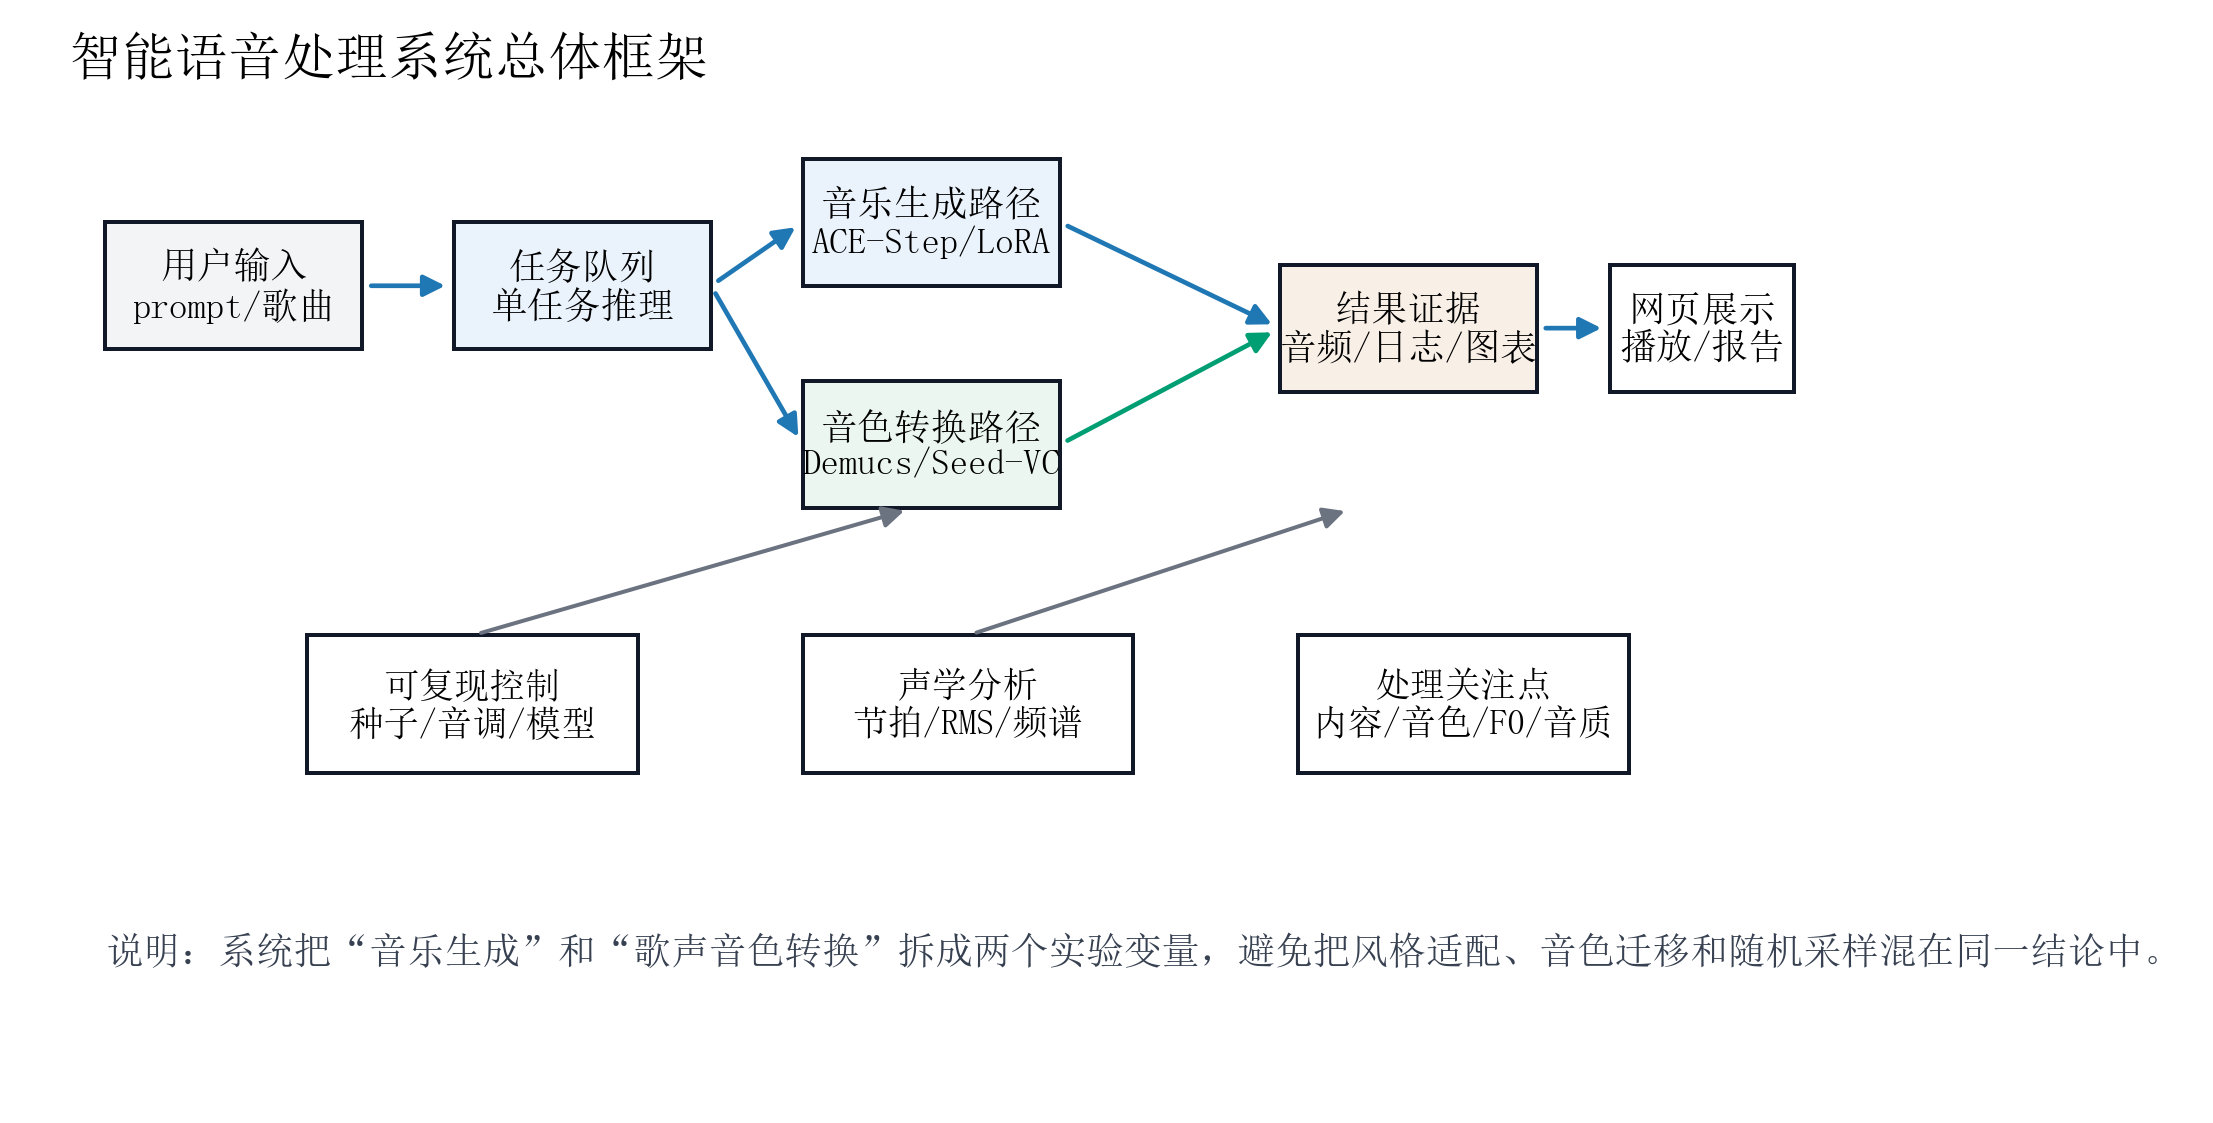
\includegraphics[width=0.92\linewidth]{assets/fig1_cn_system_architecture.png}
\caption{系统总体架构。系统将 ACE-Step 音乐生成路径和授权音色转换路径分离，实现任务队列、输出证据和网页展示的统一管理。}
\end{figure}
\section{背景与问题定义}
TTS、文本生成音乐和歌声音色转换容易被混淆，但三者的输入输出约束不同。TTS 通常从文本生成朗读语音，不需要严格匹配某首歌曲的旋律；文本生成音乐从 prompt、歌词和随机种子生成新的音乐波形，关注风格、结构和混音；歌声音色转换则要求在已有歌曲上保持内容和 F0，仅替换目标音色。若用 TTS 先生成一句目标声音再拼接到歌曲中，歌词时长、元音延展、音高滑音和小节边界都会与原曲错位，因此不适合处理完整歌曲的音色迁移。

\begin{table}[H]
\centering
\caption{智能语音处理视角下三类任务的差异}
\small
\begin{tabular}{p{0.22\linewidth}p{0.32\linewidth}p{0.36\linewidth}}
\toprule
任务类型 & 核心输入 & 关键约束 \\
\midrule
文本转语音 TTS & 文本、说话人或音色条件 & 生成朗读语音，不保证与歌曲旋律、节拍和元音时长对齐 \\
文本生成音乐 & prompt、歌词、seed、可选 LoRA & 生成新的音乐结构，可通过同 seed baseline 判断风格适配差异 \\
歌声音色转换 & 源歌曲、人声内容、F0、授权目标音色 & 保持歌词时序和旋律走势，只改变声学音色，并与伴奏重新混合 \\
\bottomrule
\end{tabular}
\end{table}
本文将授权歌声音色转换定义为条件波形重建问题。给定源音频 x、目标音色参考 r 和可选半音偏移 Δp，系统从 x 中估计内容表征 C(x) 与基频 F0(x)，从 r 中提取音色嵌入 e(r)，再由 Seed-VC 和声码器生成转换波形 y\_vc。该定义使智能语音处理中的四个因素可分开讨论：内容是否保持、音高是否稳定、目标音色是否接近、输出音质是否存在声码器伪影。

\begin{figure}[H]
\centering
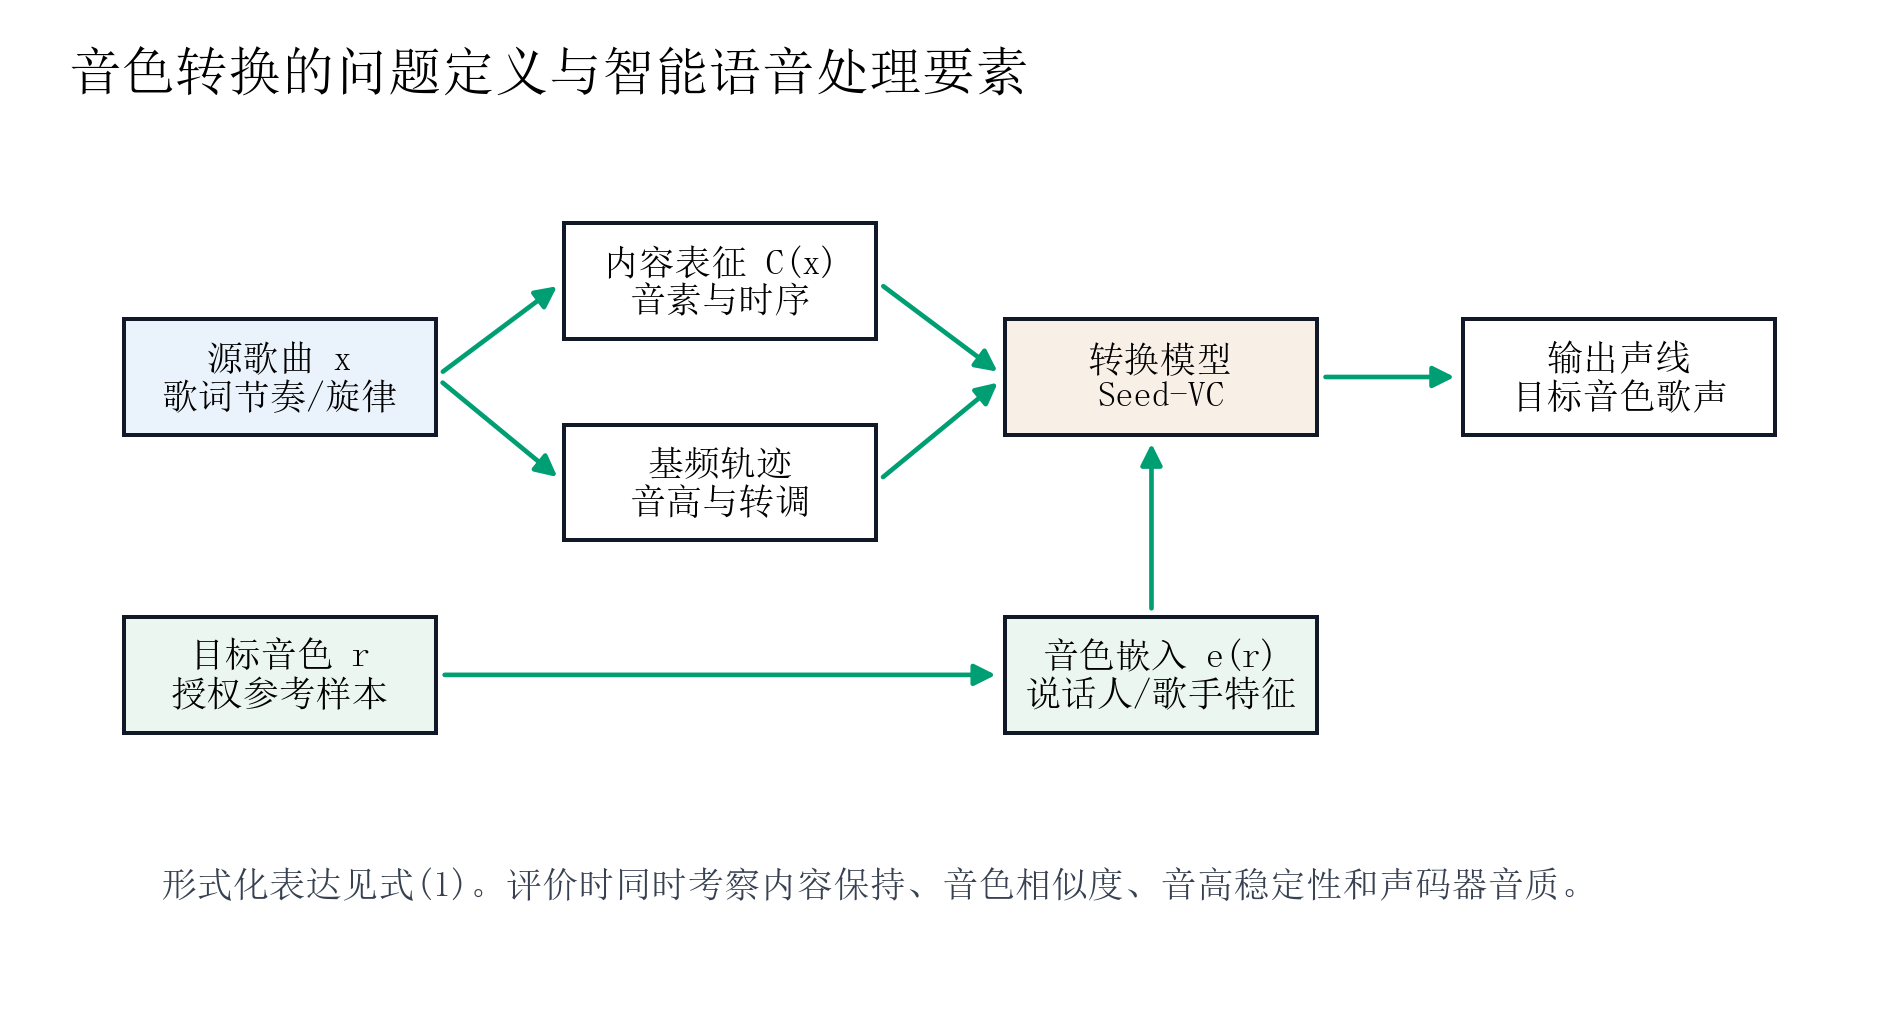
\includegraphics[width=0.92\linewidth]{assets/fig2_cn_isp_task_definition.png}
\caption{授权音色转换的问题定义。源歌曲提供内容与 F0，目标参考样本提供音色嵌入，声码器负责重建目标声线。}
\end{figure}
\begin{equation}
y_{vc}=\mathrm{Vocoder}\left(f_{\mathrm{SeedVC}}(C(x),F_0(x)+\Delta p,e(r))\right)
\end{equation}
\section{系统实现}
\subsection{LoRA 音乐生成路径}
音乐生成路径使用 ACE-Step 作为基础模型，数据侧包含 6016 条 8 秒 EDM 训练片段，训练/验证/测试划分为 4833/557/626。LoRA 从 step=960 继续训练 240 个本地 step 至 step=1200，可训练范围扩展到最后 2 个 Transformer block，可训练参数约 1.12M。网页端保留同 seed baseline 对照：在同一 prompt、seed、scheduler、采样步数和后处理参数下，分别生成 LoRA 与 ACE-Step base 音频，从而避免把随机采样差异误认为模型适配效果。

\begin{figure}[H]
\centering
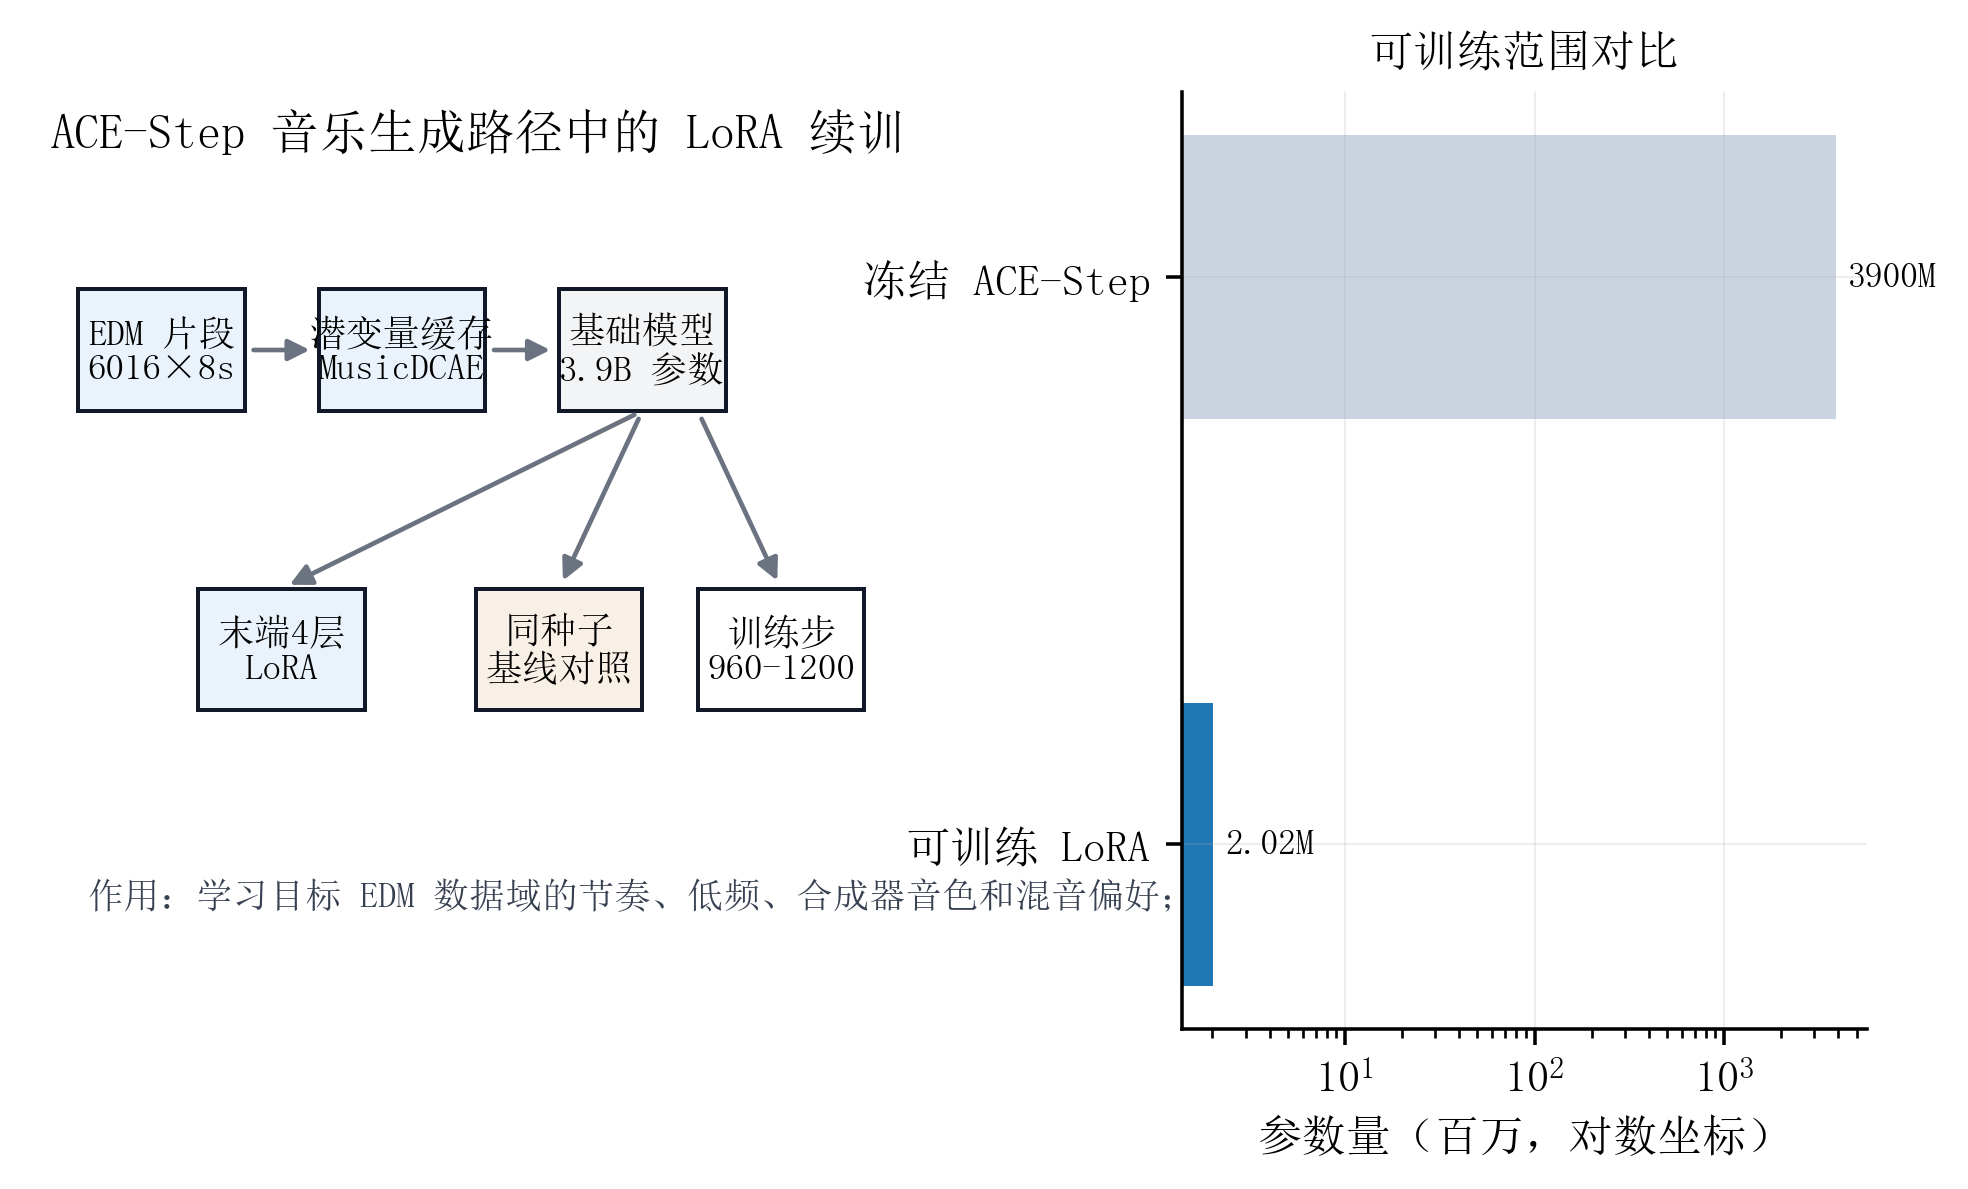
\includegraphics[width=0.92\linewidth]{assets/fig3_cn_lora_scope.png}
\caption{LoRA 音乐生成路径。LoRA 只更新少量末端参数，生成效果通过同 seed baseline 进行控制变量对照。}
\end{figure}
\subsection{授权音色转换路径}
授权音色转换路径包含上传建档、音频标准化、可选分轨、目标音色推理、伴奏重混和证据保存六个阶段。网页收到上传歌曲后，首先将原始文件复制到任务目录，记录 model\_dir、pitch\_shift、diffusion\_steps、CFG、dehiss\_strength 和 emotion\_strength 等参数，并写入 task.json 与 task.log；随后将音频转换为统一采样率和单/双声道格式，保证 Demucs 与 Seed-VC 的输入一致。分轨阶段调用 Demucs 输出 vocals、drums、bass 和 other，其中 vocals 表示待转换的人声主轨，drums、bass、other 用于合成伴奏。若 vocals stem 存在，Seed-VC 只处理人声，转换后人声再与 accompaniment 相加并峰值归一化，得到新的完整歌曲；若分轨失败，系统明确记录警告并退回整曲转换，避免静默产生不可解释结果。

\begin{figure}[H]
\centering
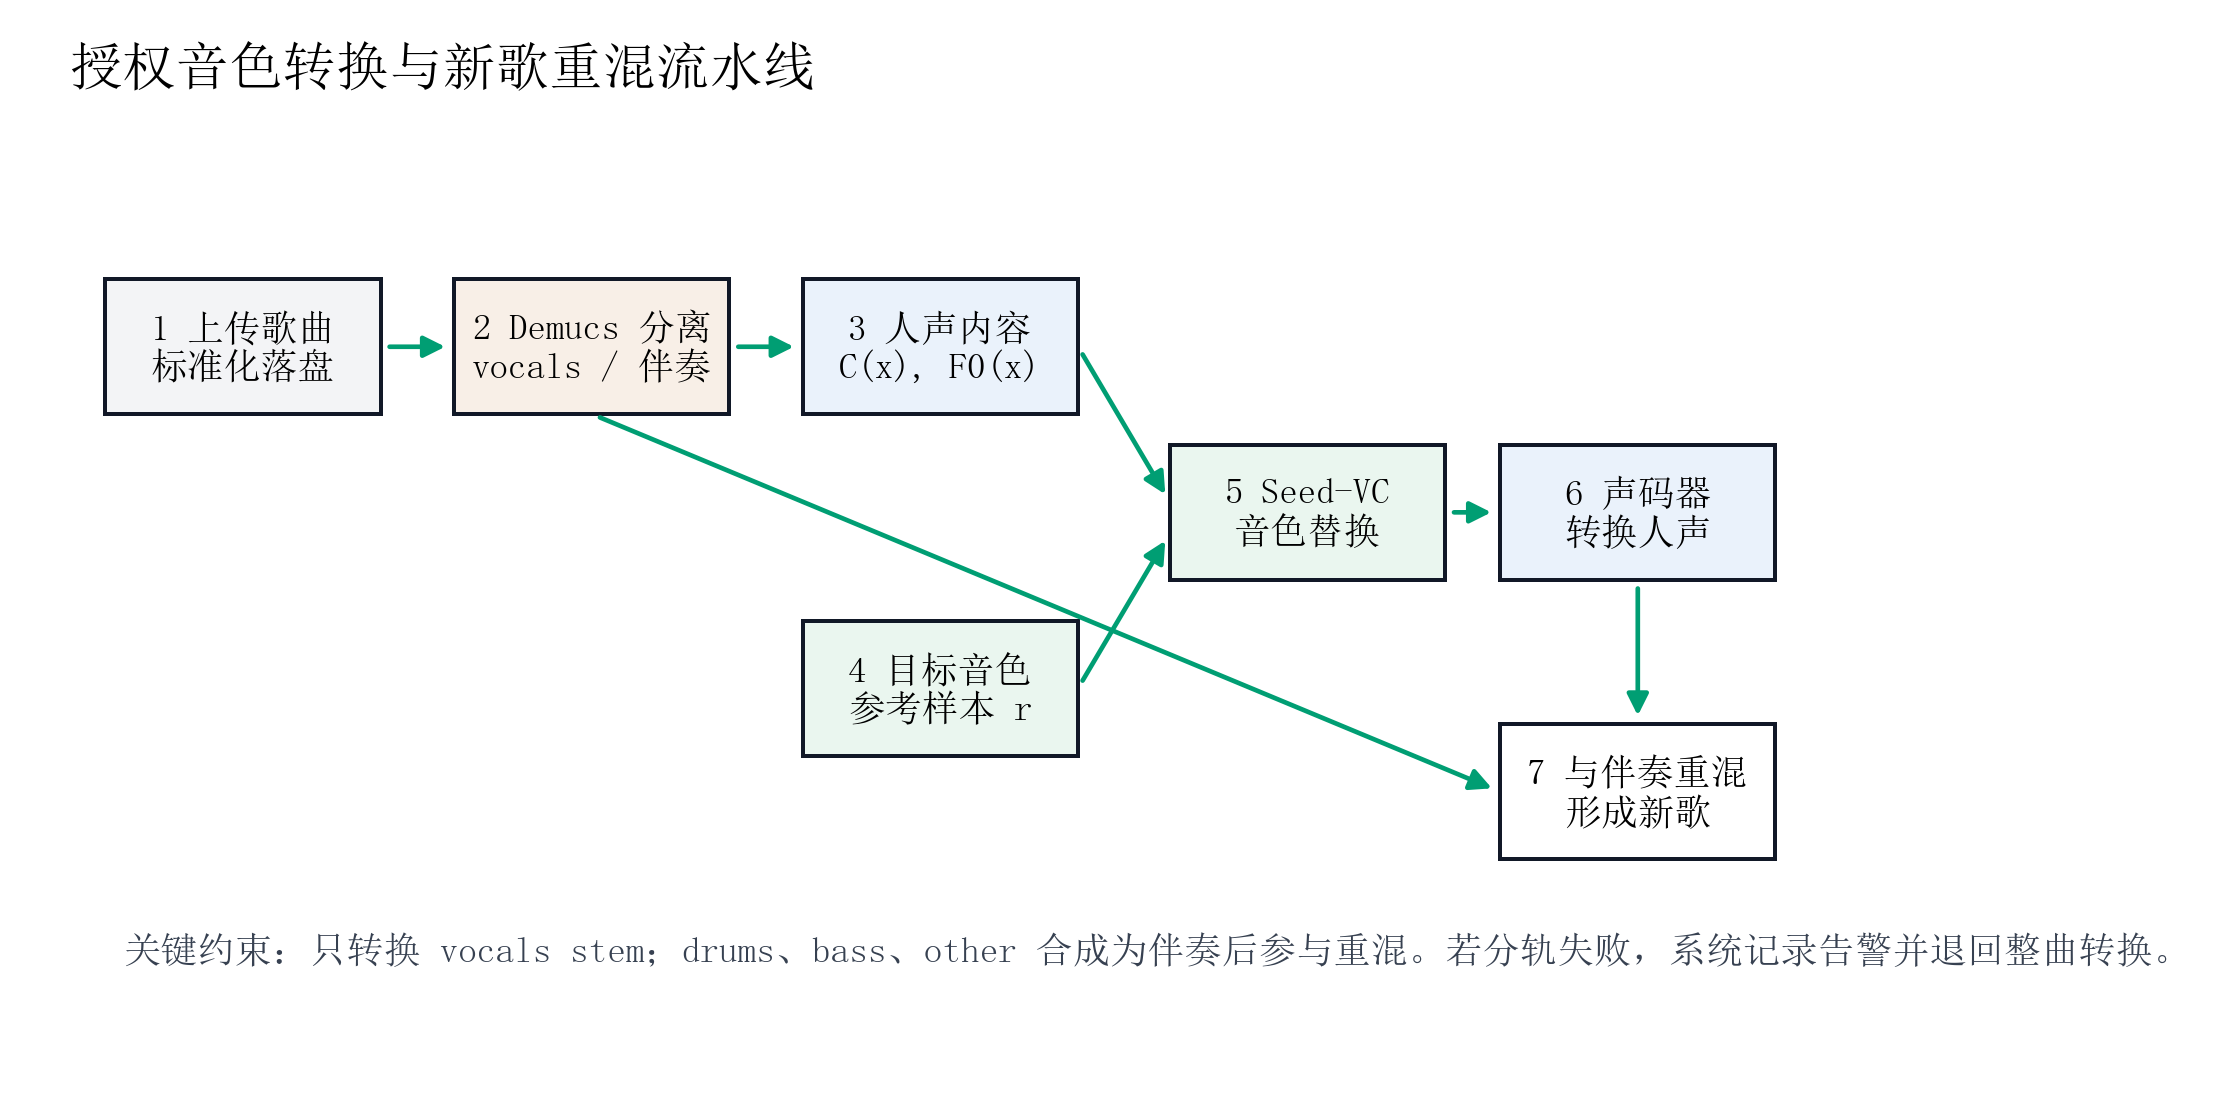
\includegraphics[width=0.92\linewidth]{assets/fig4_cn_voice_conversion_pipeline.png}
\caption{授权音色转换与新歌重混流水线。系统先分离人声与伴奏，再完成音色替换和重混。}
\end{figure}
\begin{equation}
y_{mix}=\mathrm{Normalize}\left(y_{vc}+g_v\cdot a\right)
\end{equation}
式中 y\_vc 为 Seed-VC 输出并经过后处理的人声，a 为由 drums、bass、other 合成的伴奏，g\_v 为网页端可调的人声重混增益。该公式对应系统实现中的最后一步：先按目标响度修正转换人声，再与伴奏对齐采样率和长度，最后进行峰值归一化，从而减少削波并保持伴奏结构。该设计使“音色替换”和“伴奏重混”在实验记录中可分开检查。

\begin{table}[H]
\centering
\caption{Web 音色转换处理流程}
\small
\begin{tabular}{p{0.22\linewidth}p{0.32\linewidth}p{0.36\linewidth}}
\toprule
阶段 & 实现方式 & 保存证据 \\
\midrule
上传与建档 & 复制 uploaded\_song.*，记录 model\_dir、pitch\_shift、任务 ID & uploaded\_song、task.json、task.log \\
人声分离 & Demucs 输出 vocals、drums、bass、other & stems 字典、四轨 wav、失败告警 \\
音色转换 & Seed-VC 使用 vocals 和目标参考样本进行零样本 SVC & converted\_vocal、converter\_stdout、seed\_vc 日志 \\
伴奏重混 & drums+bass+other 合成伴奏，再与 converted\_vocal 混合 & accompaniment、voice\_conversion\_mix \\
结果诊断 & 提取 BPM、RMS、低频比例、频谱质心和起音密度 & analysis.txt、波形/频谱 PNG \\
\bottomrule
\end{tabular}
\end{table}
\begin{table}[H]
\centering
\caption{授权音色转换与伴奏重混流程}
\small
\begin{tabular}{p{0.22\linewidth}p{0.32\linewidth}p{0.36\linewidth}}
\toprule
步骤 & 输入 & 操作 \\
\midrule
1 & 上传歌曲 x、目标音色目录 r & 建立任务目录，写入参数、时间戳和原始输入 \\
2 & uploaded\_song.* & 调用 Demucs；若 vocals 存在，则把 vocals 作为转换源 \\
3 & vocals、pitch shift Δp & 执行轻量去沙预处理，减少分轨残留高频噪声 \\
4 & 清理后 vocals、目标参考样本 & 调用 Seed-VC，设置扩散步数、CFG、F0 条件和半音偏移 \\
5 & converted\_vocal\_raw & 按去沙强度与情感力度系数做后处理和响度修正 \\
6 & converted\_vocal、accompaniment & 重混并生成新歌，保存 waveform、analysis 和文件清单 \\
\bottomrule
\end{tabular}
\end{table}
\subsection{模型来源与本地桥接}
本地 ckpt/pth 文件更接近 GPT-SoVITS TTS 组合，不能直接解释为歌曲 VC 推理入口。本文采用 Seed-VC 作为零样本歌声音色转换工具，并编写本地 wrapper 统一 source、output、pitch、model\_dir 和 task\_dir 参数。另一方面，Demucs 安装在 edm-adapter conda 环境中，而网页进程可能运行在 base Python；为保证可用性，分离 wrapper 在当前解释器缺少 demucs 时自动切换到 conda run -n edm-adapter 执行。这一桥接方式避免了在 Gradio 进程中常驻多个大模型，也使后续替换为 RVC/SVC 等其他授权转换器时只需替换命令模板。

\begin{table}[H]
\centering
\caption{模型来源与本地证据}
\small
\begin{tabular}{p{0.22\linewidth}p{0.32\linewidth}p{0.36\linewidth}}
\toprule
模块 & 来源或路径 & 作用 \\
\midrule
ACE-Step & 本地基础模型缓存 & 文本到音乐生成基础模型 \\
LoRA adapter & outputs/avicii\_local\_lora/... & 目标 EDM 风格适配 \\
Demucs & conda env: edm-adapter & 分离 vocals、drums、bass、other \\
Seed-VC & external\_tools/seed-vc & 零样本歌声音色转换 \\
目标音色样本 & 凄く苦そうだけど……美味しいじゃあ、どうして…….wav & 授权目标音色参考，不在论文中硬编码人物身份 \\
\bottomrule
\end{tabular}
\end{table}
\subsection{任务队列与证据链设计}
为降低网页交互与模型推理之间的耦合，系统采用任务队列方式组织实验。每次提交都会生成唯一任务 ID，并在 outputs/web\_generations 下建立独立目录；网页只负责提交参数、轮询状态和展示产物，实际推理在后台工作线程中执行。这种设计的优点是模型调用失败、分轨失败或后处理异常都不会破坏前端会话，且每个阶段的中间文件都可被再次检查。在资源管理上，系统默认限制同类重任务并发数量，避免同时加载多个分离模型或转换模型造成内存峰值过高。

\begin{table}[H]
\centering
\caption{任务目录中的证据链文件}
\small
\begin{tabular}{p{0.22\linewidth}p{0.32\linewidth}p{0.36\linewidth}}
\toprule
文件或目录 & 产生阶段 & 科研用途 \\
\midrule
uploaded\_song.* & 上传建档 & 保存原始输入，保证后续实验可回放 \\
htdemucs/.../vocals.wav & 人声分离 & 检查待转换人声是否干净，判断伴奏泄漏 \\
accompaniment\_*.wav & 伴奏合成 & 验证 drums、bass、other 是否被正确重混 \\
converted\_vocal\_raw\_*.wav & Seed-VC 推理 & 与后处理版本对照，定位声码器伪影 \\
converted\_vocal\_*.wav & 去沙与包络修正 & 分析 dehiss\_strength 与 emotion\_strength 的影响 \\
voice\_conversion\_mix\_*.wav & 伴奏重混 & 作为最终听评和客观指标计算对象 \\
task.json / task.log & 全流程记录 & 追溯参数、命令、耗时、状态和错误信息 \\
\bottomrule
\end{tabular}
\end{table}
\section{实验与结果}
\subsection{实验流程与参数设置}
实验过程分为音乐生成对照实验和歌声音色转换实验两组。音乐生成对照实验固定 prompt、seed、duration、infer\_step 和 guidance，只切换是否加载 LoRA adapter，用于判断目标 EDM 数据域适配是否改变同一随机起点下的生成分布。歌声音色转换实验固定上传歌曲、目标音色目录和分轨策略，依次记录 Demucs 分离结果、Seed-VC 原始输出、去沙/包络修正后人声以及伴奏重混结果。所有实验均以任务目录为最小复现实验单元，正文中的图表均来自该目录下的 wav、png、json 和 log 文件。

\begin{table}[H]
\centering
\caption{实验过程与记录内容}
\small
\begin{tabular}{p{0.22\linewidth}p{0.32\linewidth}p{0.36\linewidth}}
\toprule
实验阶段 & 主要操作 & 记录内容 \\
\midrule
E1 输入规范化 & 复制上传歌曲，统一采样率、声道和文件命名 & uploaded\_song、任务 ID、输入时长 \\
E2 人声/伴奏分离 & 调用 Demucs 生成 vocals、drums、bass、other & 四轨 wav、accompaniment、分轨告警 \\
E3 音色转换 & 将 vocals 与授权参考样本输入 Seed-VC，设置 pitch、CFG 和扩散步数 & converted\_vocal\_raw、转换日志、RTF \\
E4 后处理与重混 & 执行去沙、包络保留、人声增益和峰值归一化 & converted\_vocal、voice\_conversion\_mix、声学指标 \\
E5 LoRA 对照 & 同 seed 生成 baseline 与 LoRA 音频 & same\_seed 对照音频、RMS、低频比例 \\
\bottomrule
\end{tabular}
\end{table}
\subsection{音色转换链路验证}
实验部分记录网页系统完成的一次短片段端到端任务，用于验证修复后的分离、转换和重混链路。任务 ID 为 20260603\_093222\_voice\_conversion\_d703c93b，输入为约 279.7 秒音频，pitch shift 设置为 0。系统成功调用 Demucs 得到 vocals、drums、bass 和 other，其中 vocals 被送入 Seed-VC 完成目标音色转换，其余三轨合成为 accompaniment，并与转换后人声重混得到新的完整歌曲。

\begin{figure}[H]
\centering
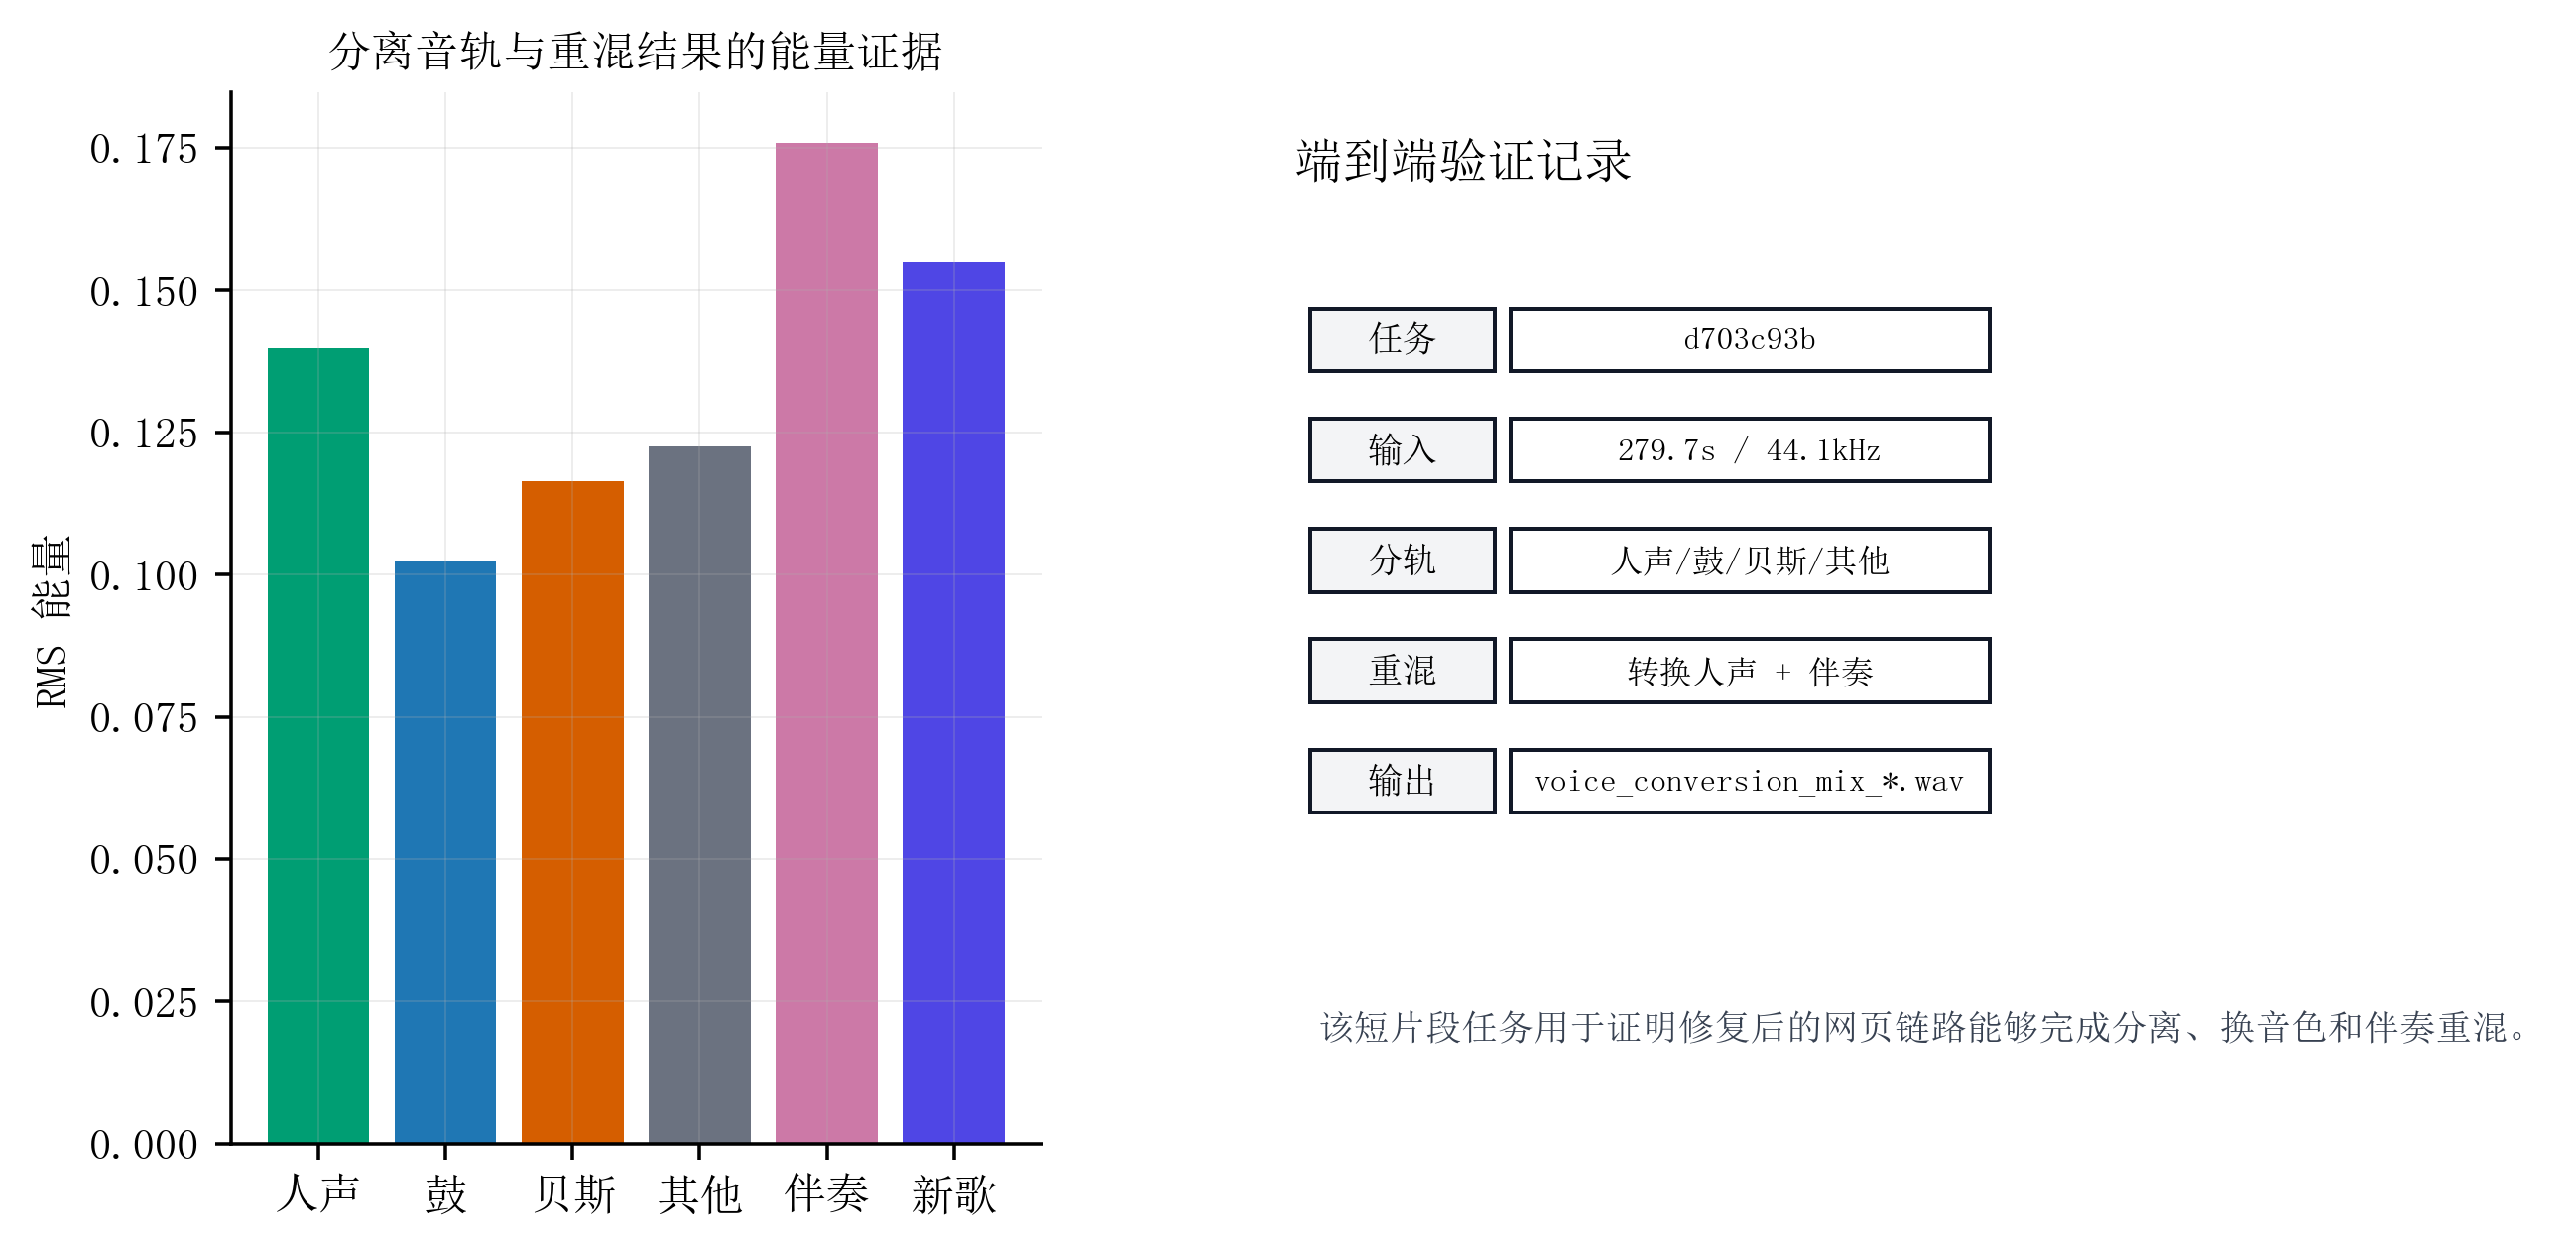
\includegraphics[width=0.92\linewidth]{assets/fig5_cn_stem_remix_evidence.png}
\caption{分离音轨与重混证据。左侧显示各 stem 与新歌输出的 RMS 能量，右侧列出任务级记录。}
\end{figure}
\begin{figure}[H]
\centering
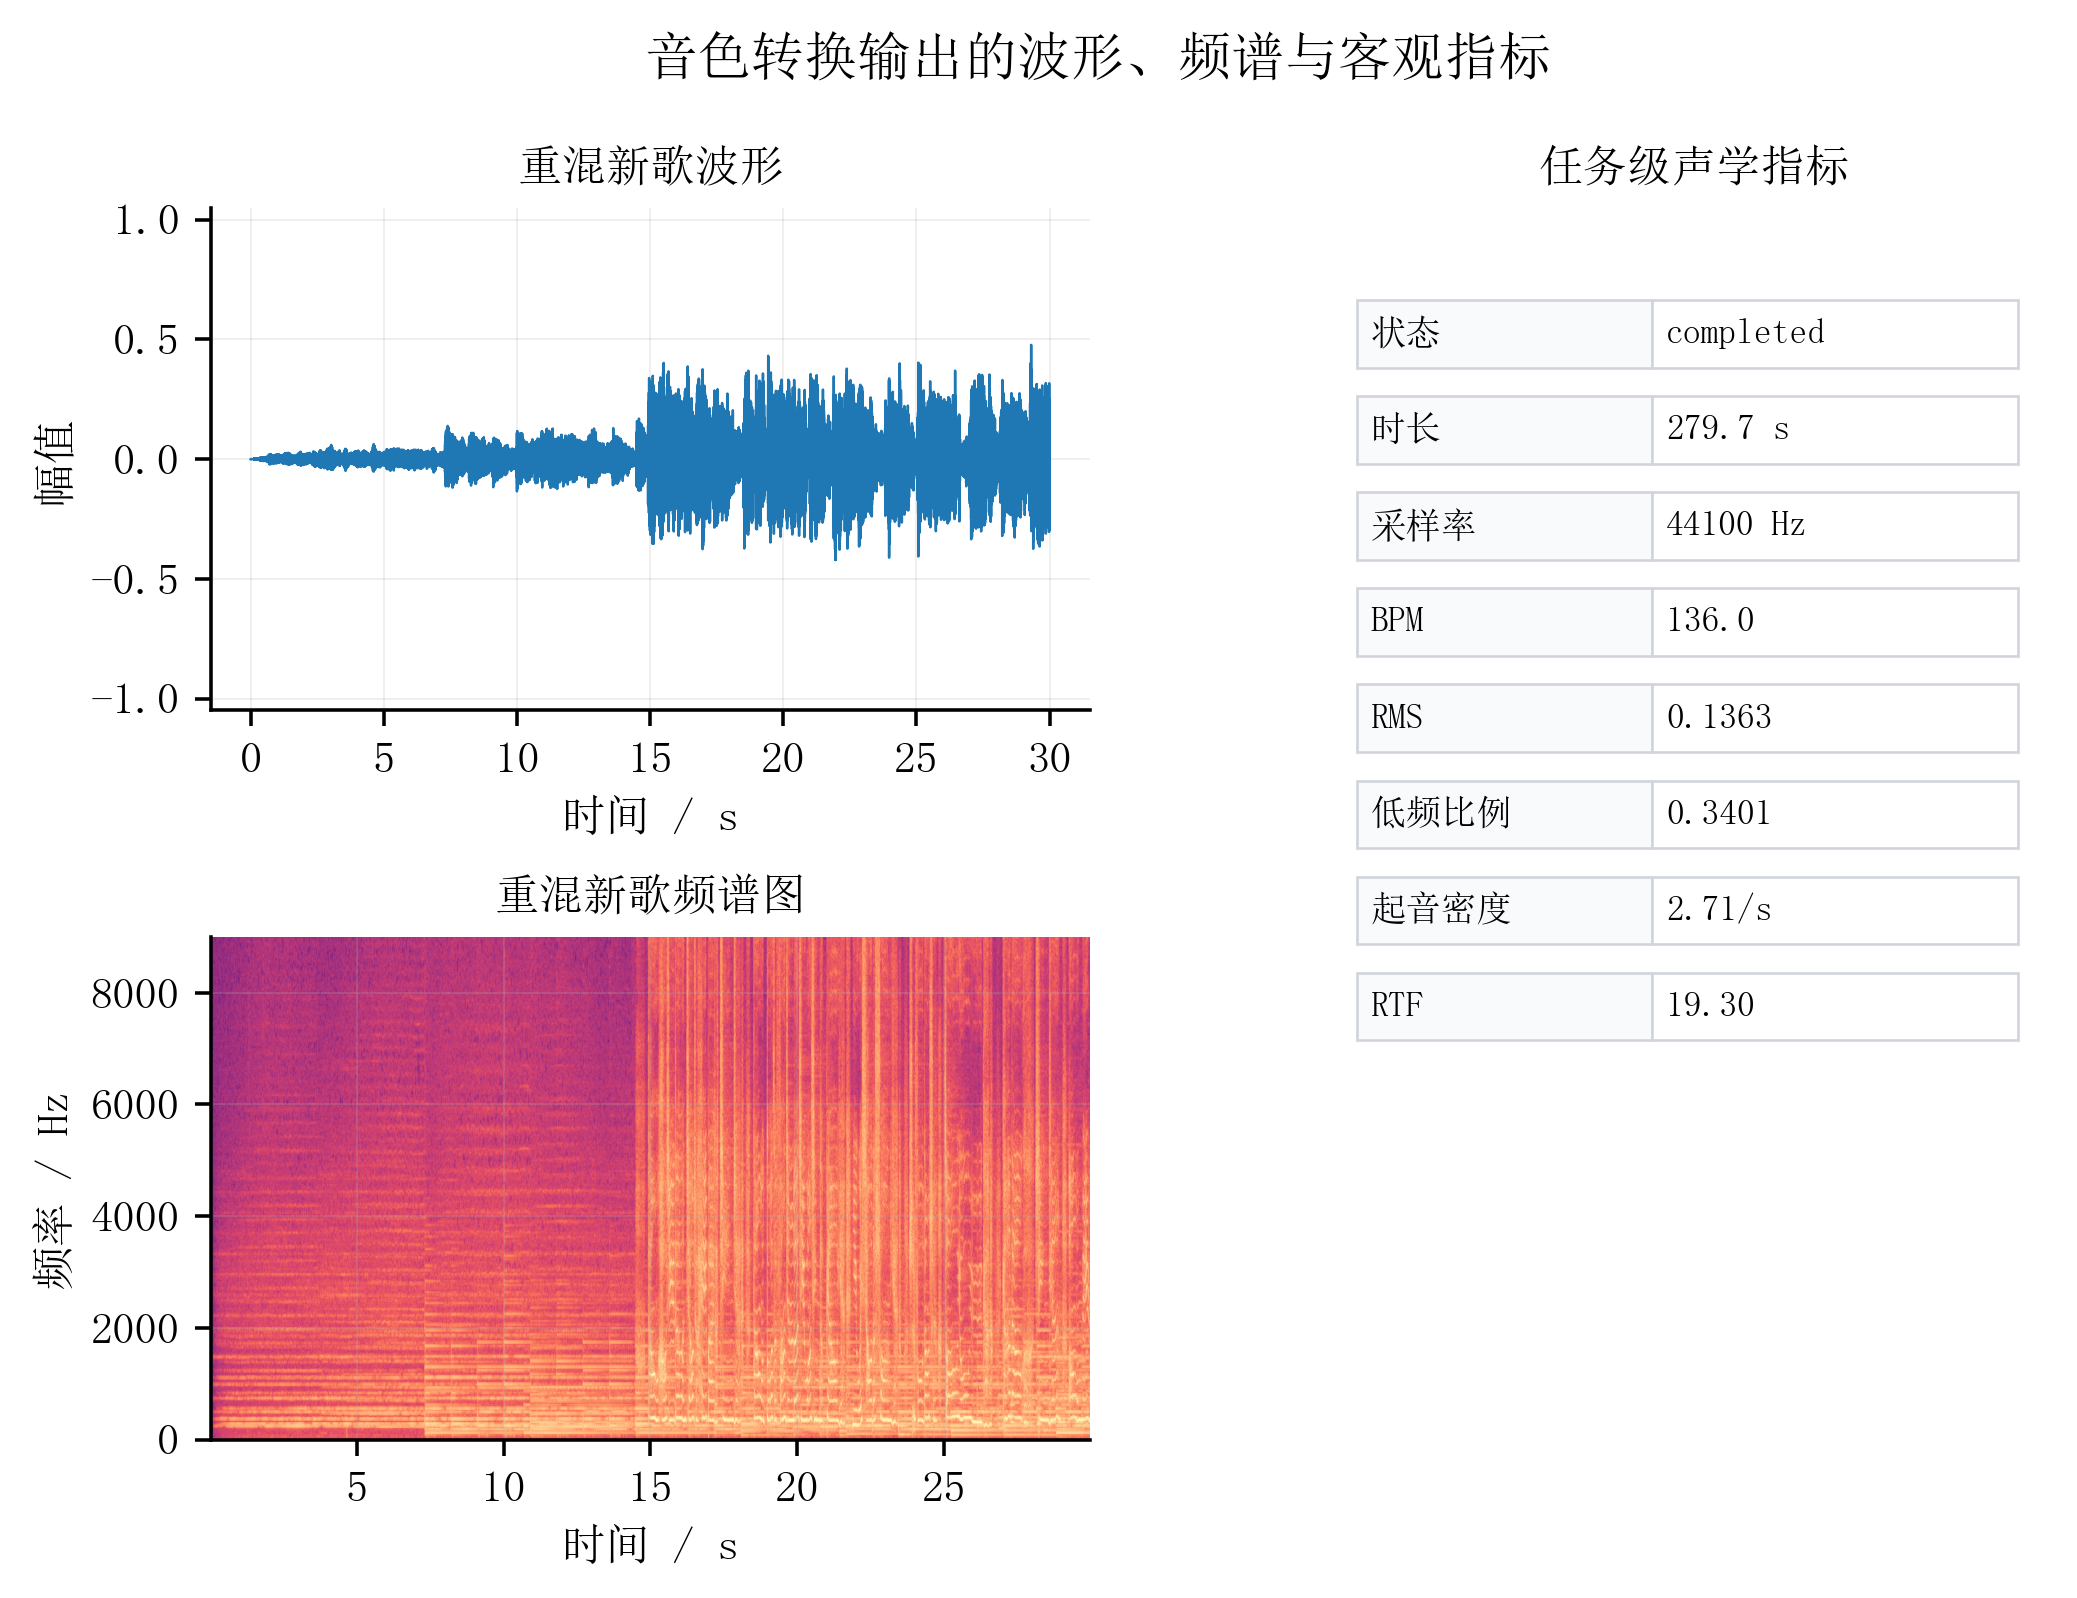
\includegraphics[width=0.92\linewidth]{assets/fig6_cn_waveform_spectrum_metrics.png}
\caption{音色转换输出的波形、频谱与客观指标。该图用于检查响度、频带分布和任务级声学指标。}
\end{figure}
\begin{table}[H]
\centering
\caption{实际网页任务的音色转换结果}
\small
\begin{tabular}{p{0.22\linewidth}p{0.32\linewidth}p{0.36\linewidth}}
\toprule
项目 & 记录 & 解释 \\
\midrule
任务 ID & 20260603\_093222\_voice\_conversion\_d703c93b & completed \\
转换输出 & voice\_conversion\_mix\_20260603\_093222\_voice\_conversion\_d703c93b.wav & 279.7s / 44100 Hz \\
分轨状态 & 已产出 vocals、drums、bass、other 并完成伴奏重混 & 用于判断是否可解释为“人声转换 + 伴奏重混” \\
声学指标 & BPM=136.0, RMS=0.1363 & 低频=0.3401, onset=2.71/s \\
推理速度 & Seed-VC 离线推理 & RTF=19.30 \\
\bottomrule
\end{tabular}
\end{table}
\begin{figure}[H]
\centering
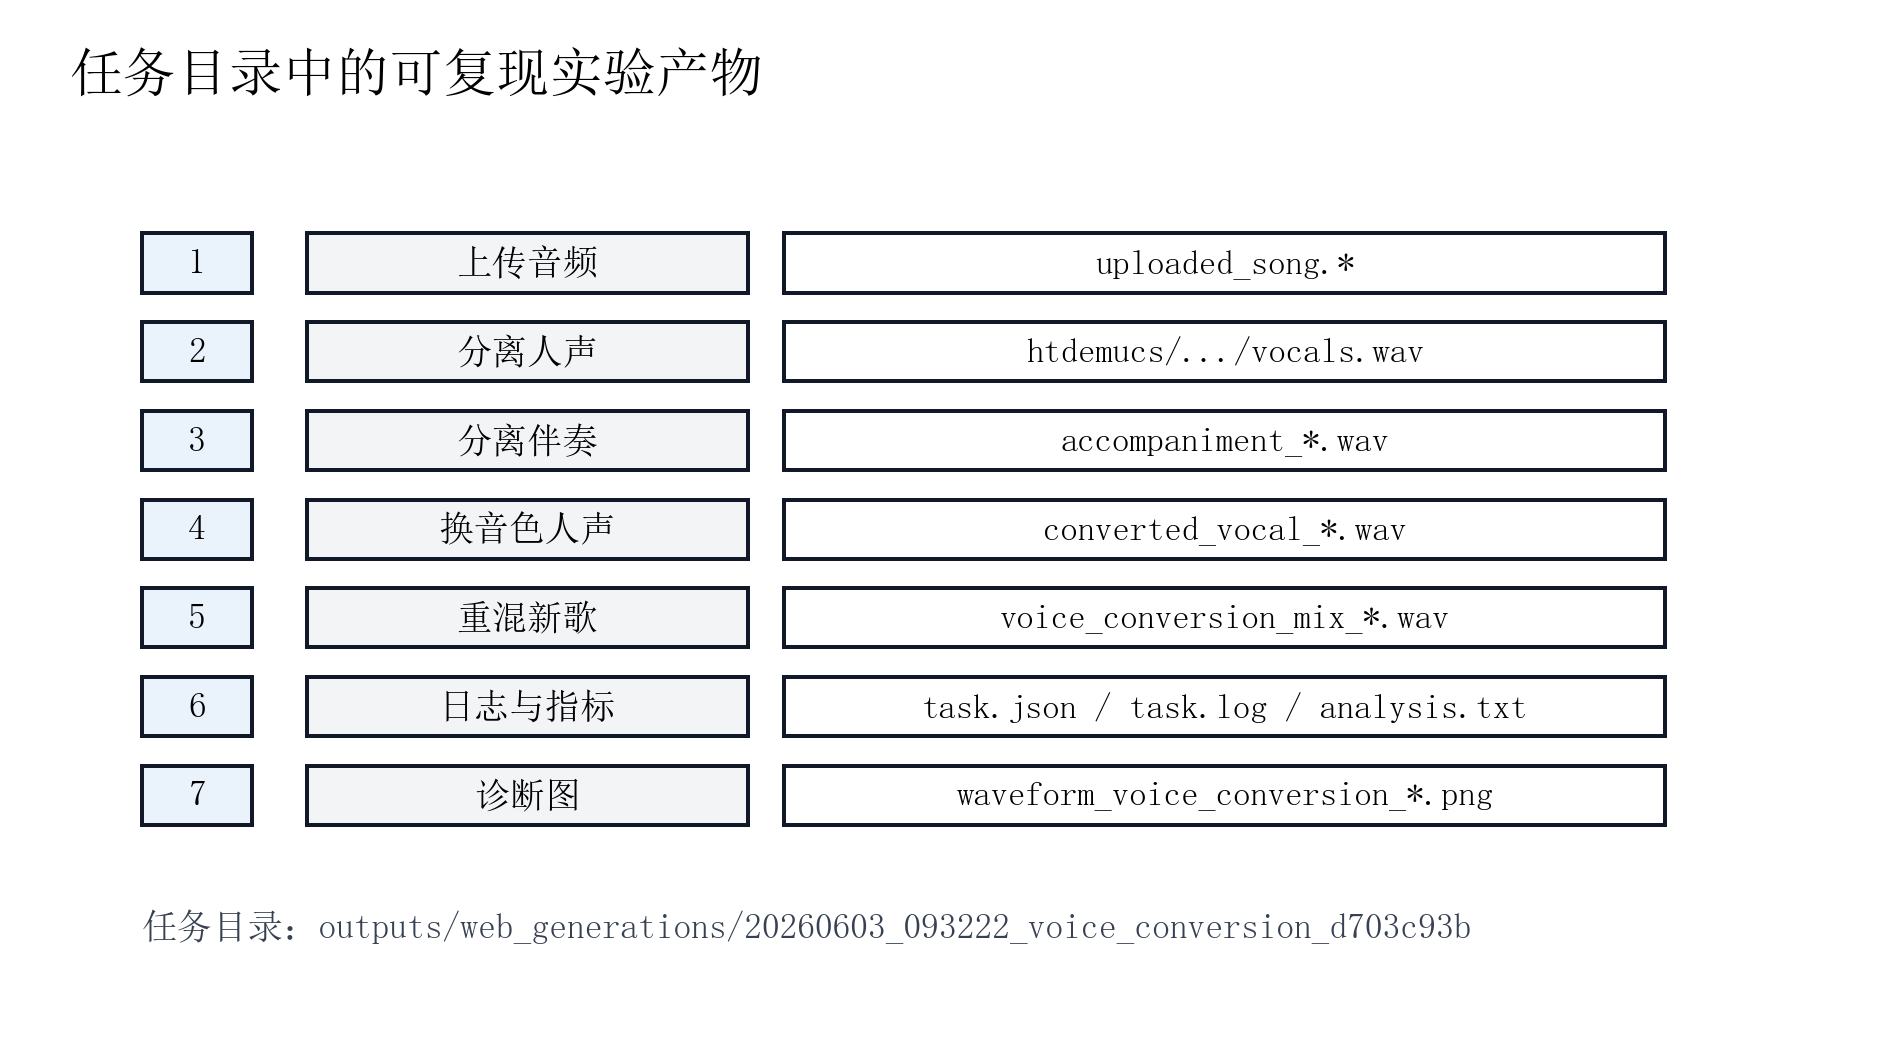
\includegraphics[width=0.92\linewidth]{assets/fig7_cn_reproducibility_records.png}
\caption{任务目录中的可复现实验产物。每个输出都可追溯到同一任务 ID、命令日志和参数记录。}
\end{figure}
从结果看，短片段链路已经能证明系统不是简单地对整曲做黑箱处理，而是具备人声分离、音色替换和伴奏重混三个可检查阶段。其中 vocals stem 的纯净程度决定转换器接收的是歌唱内容还是混入伴奏的复合信号；converted\_vocal\_raw 与后处理版本的对照用于定位沙哑和高频毛刺；最终 mix 的 RMS、低频比例和起音密度用于检查人声是否被伴奏盖住以及重混是否产生明显失衡。对于完整歌曲，系统更适合采用“短片段筛选参数、整曲离线复核”的实验流程，先确定 pitch、CFG、去沙和人声增益，再提交长音频任务。

\subsection{生成音乐路径的基线对照}
LoRA 音乐生成路径仍保留为系统的另一条智能音频处理证据。与音色转换不同，LoRA 关注的是生成分布是否向目标 EDM 风格移动。因此，本文不使用音色转换任务的主观听感来评价 LoRA，而采用同 seed baseline 生成的客观诊断指标进行控制变量比较。该设计使音乐生成和歌声音色转换在评价问题上保持清晰边界。

\begin{figure}[H]
\centering
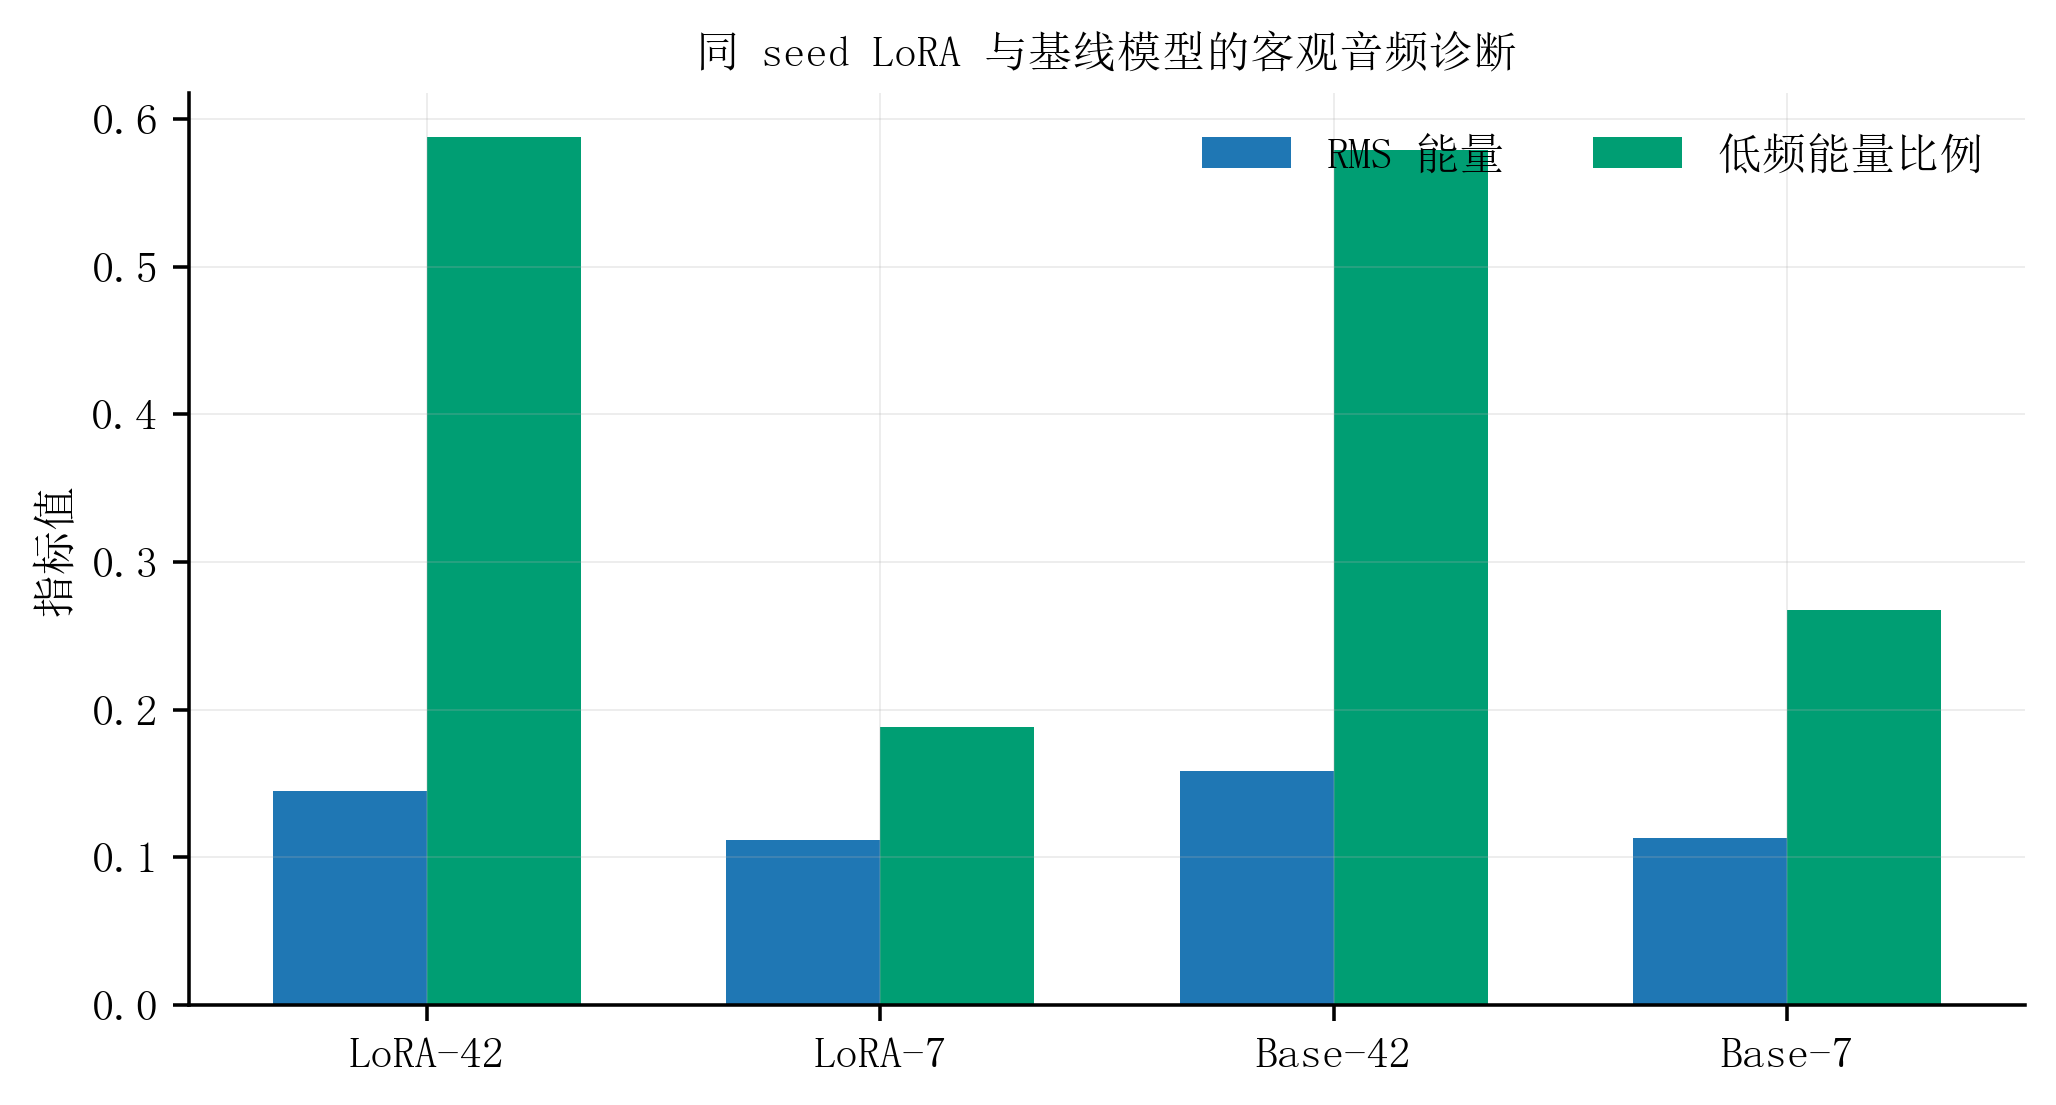
\includegraphics[width=0.92\linewidth]{assets/fig8_cn_lora_baseline_metrics.png}
\caption{同 seed LoRA 与 baseline 的客观音频诊断。该图作为音乐生成路径的基线证据，与音色转换路径分开解释。}
\end{figure}
\subsection{评价协议与资源预算分析}
为了使实验结论具备会议论文所需的可解释性，本文不把不同任务的输出混成一个总评分。音乐生成实验只改变 LoRA 开关；音色转换实验只改变目标音色、转调和后处理参数；音质修复实验只比较 Seed-VC raw 与后处理输出。这种设计虽然不会立即给出一个“最好听”的单指标排名，但能明确说明每个模块到底在影响什么。

\begin{figure}[H]
\centering
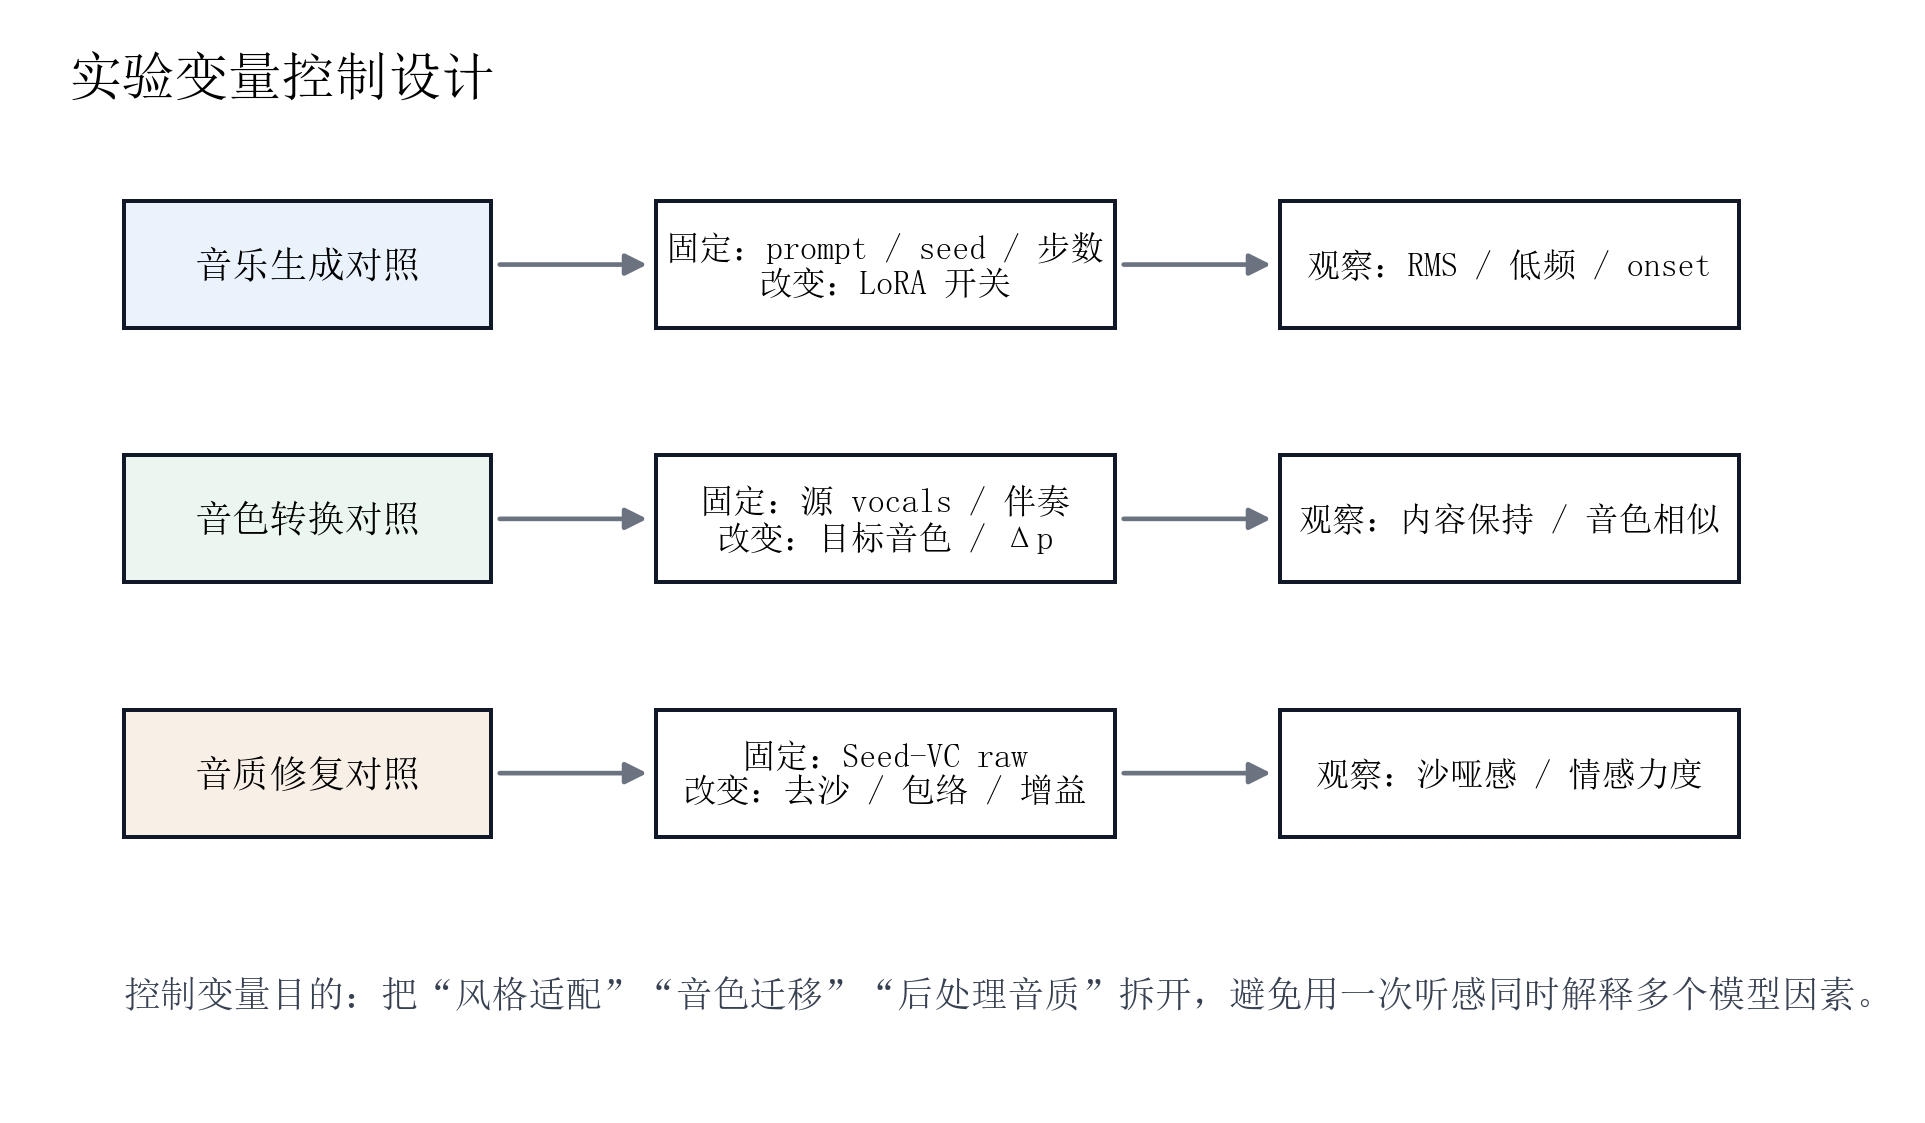
\includegraphics[width=0.92\linewidth]{assets/fig9_cn_experiment_control_matrix.png}
\caption{实验变量控制矩阵。系统将 LoRA 生成、歌声音色转换和后处理音质修复拆成三个独立评价对象。}
\end{figure}
\begin{table}[H]
\centering
\caption{实验变量与控制项}
\small
\begin{tabular}{p{0.22\linewidth}p{0.32\linewidth}p{0.36\linewidth}}
\toprule
实验对象 & 固定条件 & 改变条件 \\
\midrule
LoRA 音乐生成 & prompt、seed、duration、infer\_step、guidance、后处理链 & 是否加载 LoRA、LoRA 权重 \\
授权音色转换 & 源人声、伴奏、目标模型目录、F0 条件 & pitch shift、目标参考样本、Seed-VC CFG \\
去沙哑后处理 & Seed-VC raw 输出、伴奏轨道、目标响度 & dehiss\_strength、emotion\_strength、人声增益 \\
长音频资源预算 & 源歌曲、目标音色、扩散步数、执行环境 & max\_vocal\_seconds、切片长度、并发数、离线队列策略 \\
\bottomrule
\end{tabular}
\end{table}
评价协议采用“客观诊断 + 产物证据 + 人工听评预留”的组合。RMS、低频比例、频谱质心和起音密度用于快速定位响度、低频堆积和瞬态异常；RTF 用于说明推理成本；任务目录中的 wav、png、json 和 log 用于追溯。最终音色相似度、情感自然度和咬字清晰度仍需要人工听评确认，因此本文把人工听评列为后续研究，而不把自动指标包装成完整主观质量结论。

\begin{figure}[H]
\centering
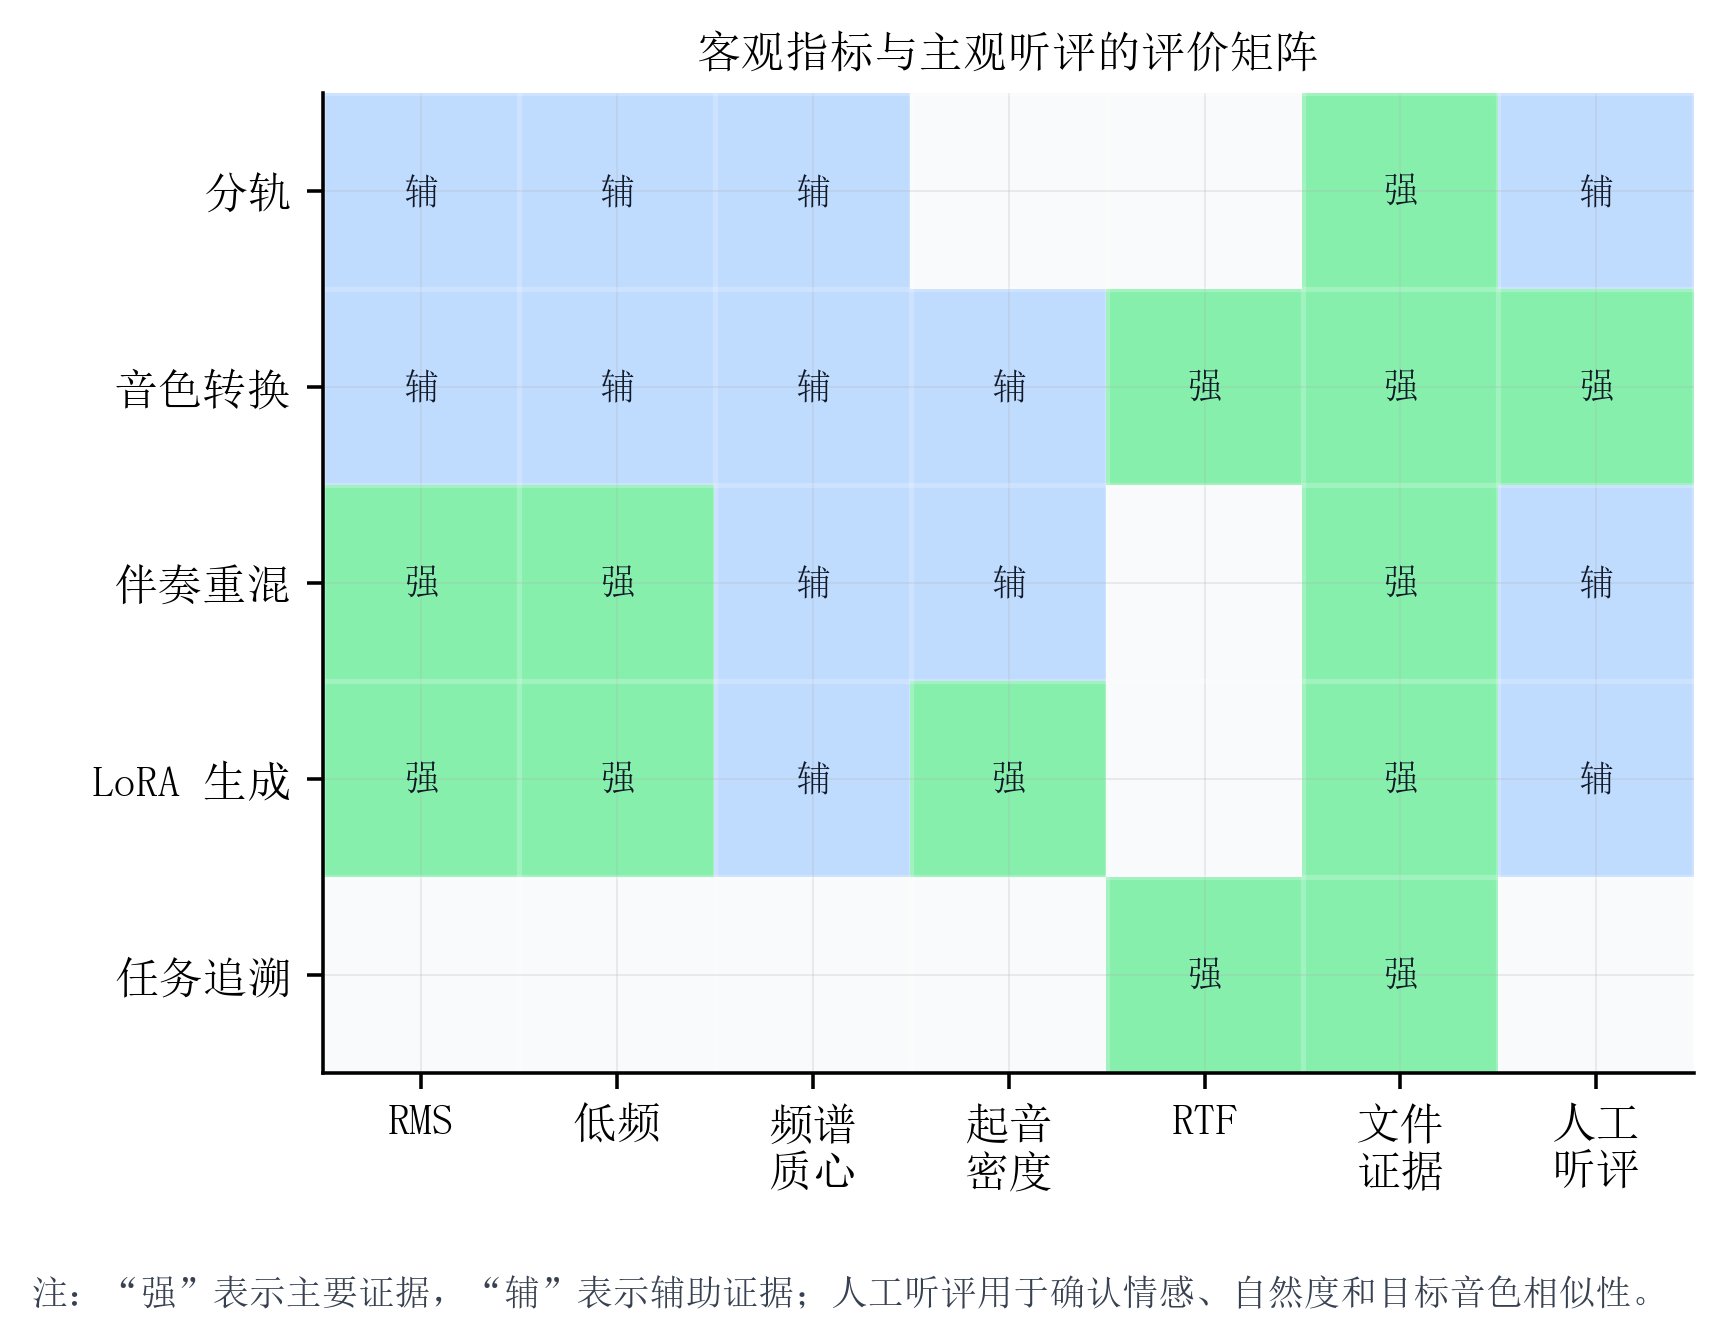
\includegraphics[width=0.92\linewidth]{assets/fig10_cn_evaluation_protocol_matrix.png}
\caption{客观指标与主观听评的评价矩阵。不同模块对应不同主证据，避免单一指标误导结论。}
\end{figure}
\begin{table}[H]
\centering
\caption{客观指标定义与用途}
\small
\begin{tabular}{p{0.22\linewidth}p{0.32\linewidth}p{0.36\linewidth}}
\toprule
指标 & 计算对象 & 解释用途 \\
\midrule
RMS & 输出波形或各 stem & 反映整体响度和重混平衡，不代表音质好坏 \\
低频比例 & 0-250 Hz 能量占比 & 定位低频堆积、伴奏泄漏和 EDM 重混低频强度 \\
频谱质心 & 短时频谱能量重心 & 辅助判断声音明暗和高频伪影 \\
起音密度 & onset 事件数量/秒 & 反映瞬态密度，适合检查节奏和分轨残留 \\
RTF & 推理耗时 / 音频时长 & 衡量是否适合实时或整曲处理 \\
任务证据 & 文件清单、日志、JSON & 确认结果是否来自同一参数和同一任务目录 \\
\bottomrule
\end{tabular}
\end{table}
长音频任务用于评估整曲处理的资源成本。当前整曲任务记录的音频时长约 279.7 秒，扩散步数为 50，CFG=0.75，系统根据短片段 RTF 与输入长度估计整曲推理耗时约 381.8 分钟。该估计不作为论文结论中的性能承诺，而作为实验调度依据：交互阶段优先使用 15 到 30 秒 vocals 片段筛选 pitch、CFG、去沙强度和重混增益，参数稳定后再提交整曲离线任务，并在 task.json 与 task.log 中记录输入长度、步数、估计耗时和实际耗时，保证长音频结果可以复核。

\begin{figure}[H]
\centering
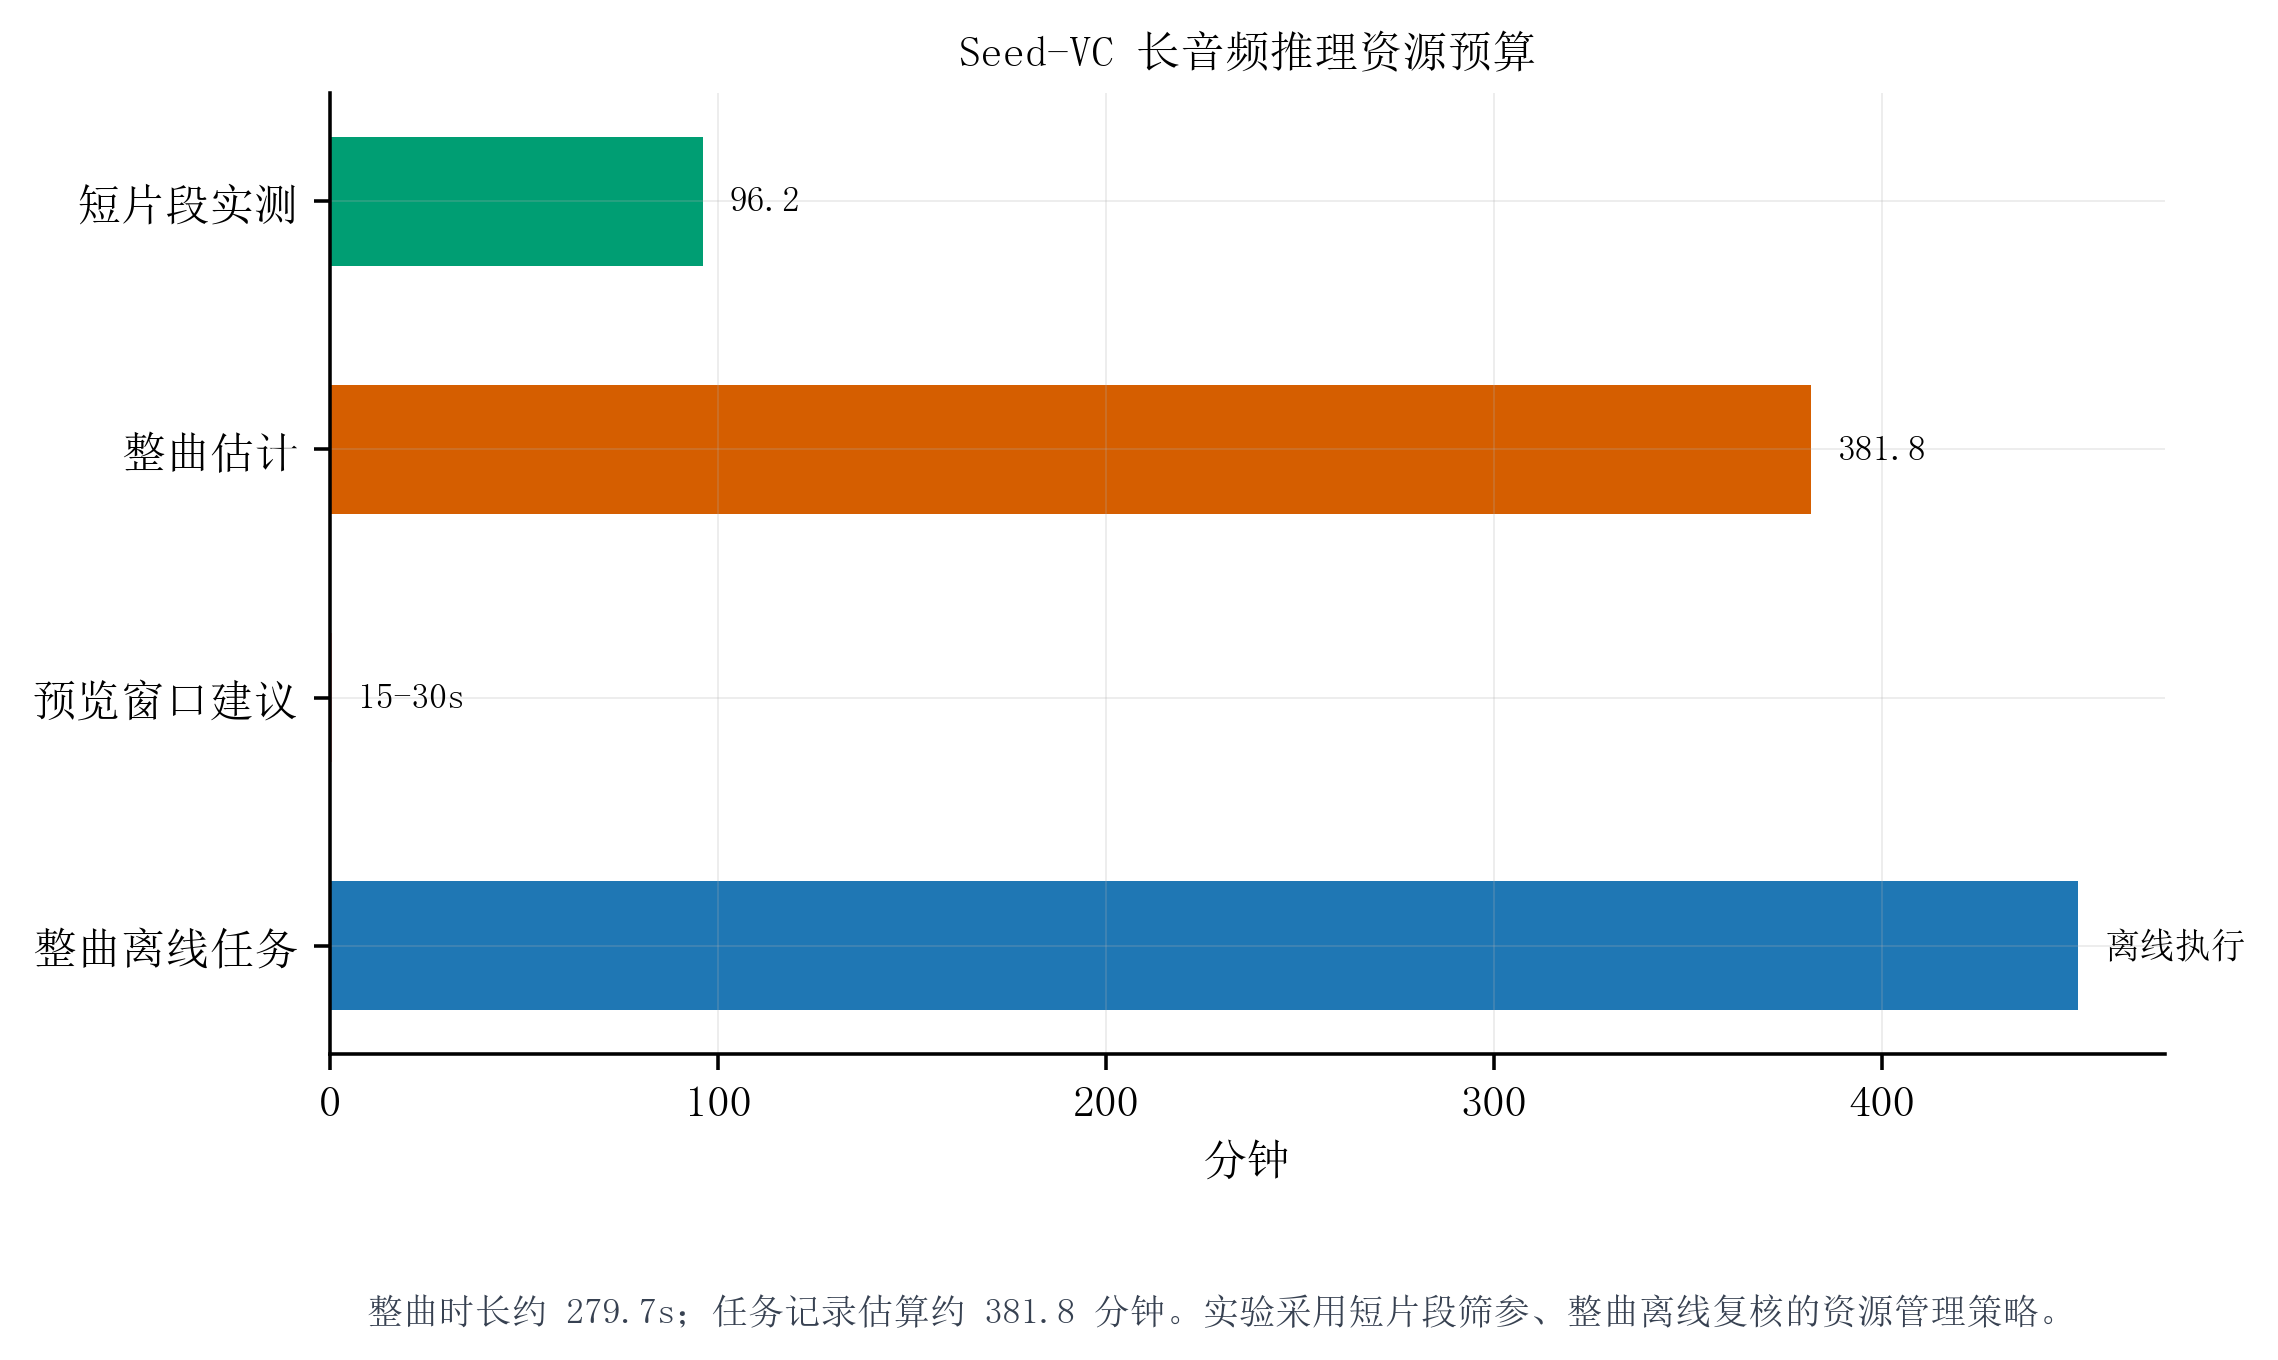
\includegraphics[width=0.92\linewidth]{assets/fig11_cn_long_audio_runtime_budget.png}
\caption{Seed-VC 长音频推理资源预算。图中对比短片段实测、整曲估计、预览窗口建议和整曲离线执行策略。}
\end{figure}
\section{讨论}
本文系统的核心价值不在于追求单次听感展示，而在于把智能语音处理任务拆成可复现的工程环节。对于歌声音色转换，授权边界要求目标音色样本必须来自用户有权使用的素材；内容边界要求 vocals stem 尽量干净，否则伴奏会被错误送入转换器；音调边界要求 pitch shift 与 F0 条件被明确记录；评价边界要求波形、频谱和客观指标不能代替最终听评，但可以帮助定位响度、低频和起音密度等明显异常。

针对用户反馈的“声音沙哑”和“情感不到位”，本文把问题拆为两类：沙哑通常来自分轨残留、声码器高频毛刺或过强的频带压缩；情感不足通常来自原人声能量包络被平滑、F0 细节被弱化或目标参考样本与歌曲情绪不匹配。当前网页暴露 dehiss\_strength=0.75、emotion\_strength=1.00、vocal\_gain\_db 等参数，并在转换前后分别做轻量去沙、包络匹配和重混增益控制。该策略不能替代更充分的目标音色样本或更高性能的推理部署，但能把可调因素暴露给实验记录。

\begin{figure}[H]
\centering
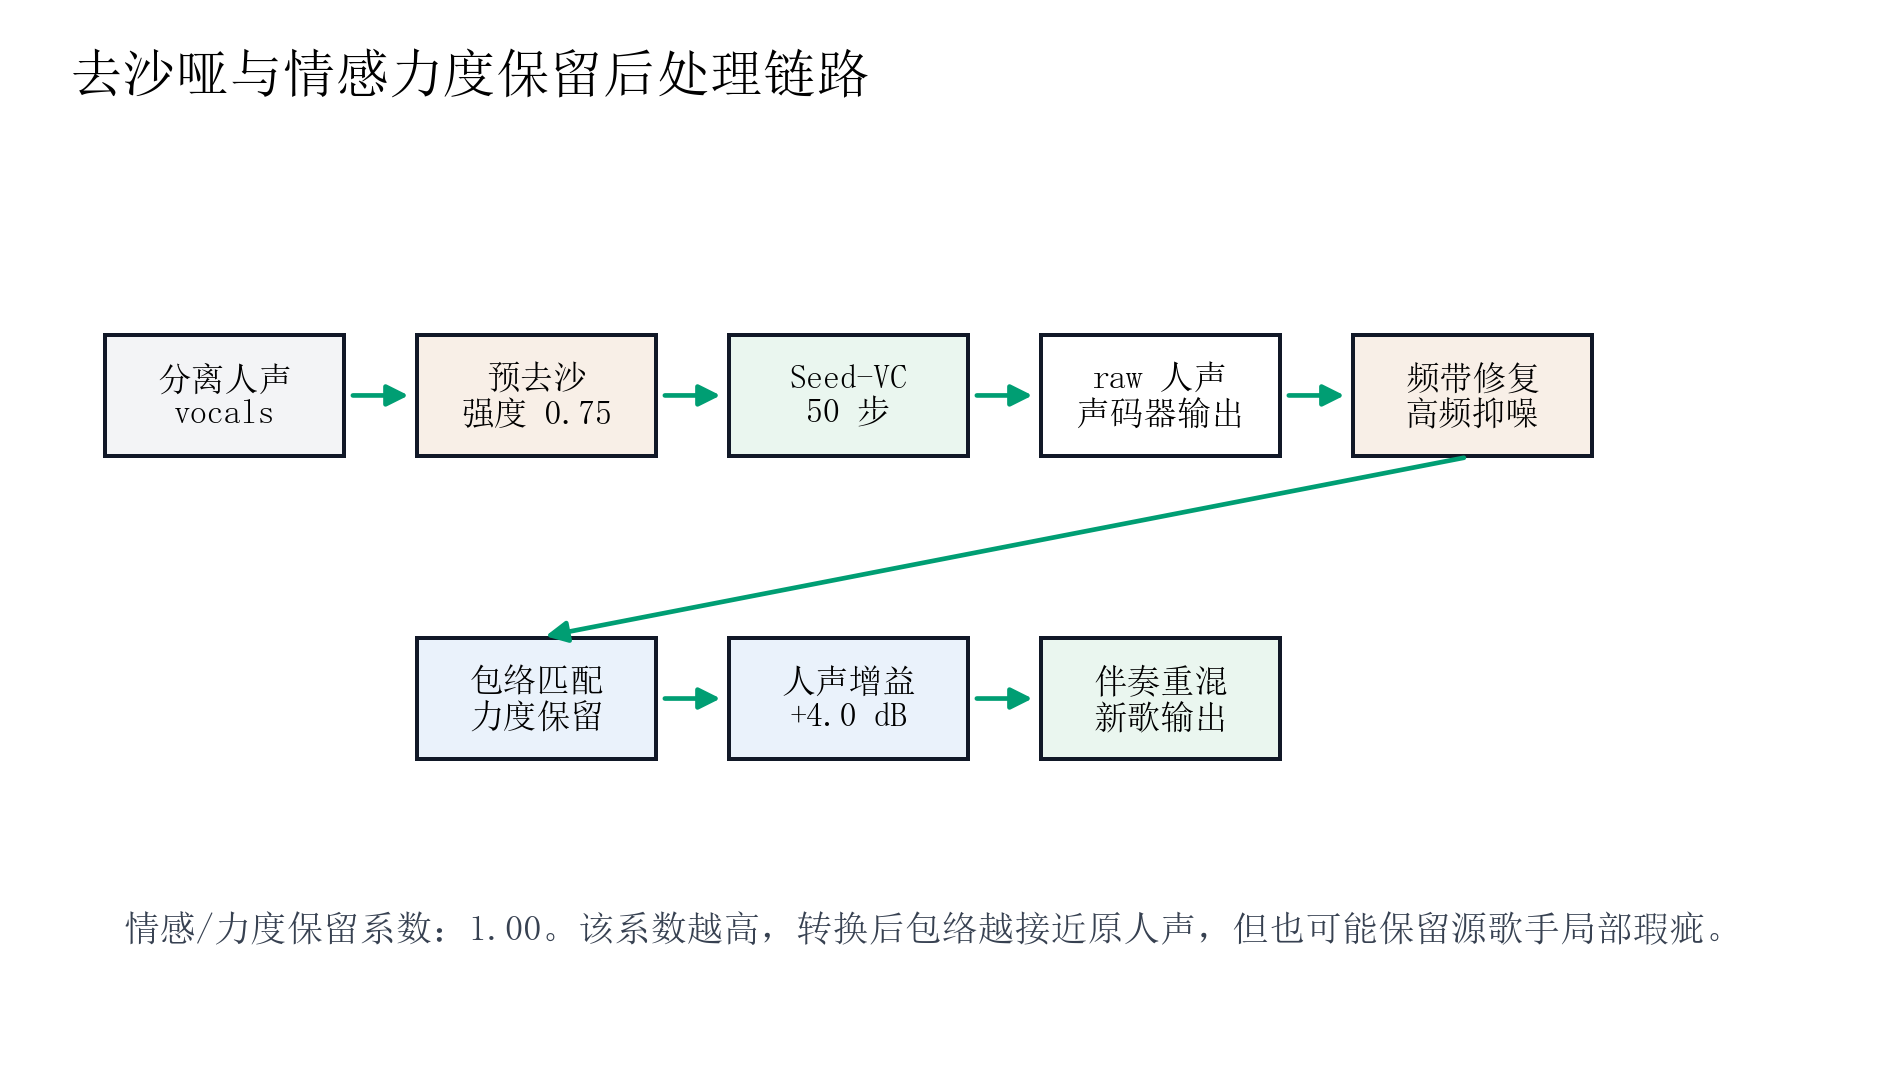
\includegraphics[width=0.92\linewidth]{assets/fig12_cn_dehiss_emotion_postprocess.png}
\caption{去沙哑与情感力度保留后处理链路。该图说明 Seed-VC raw 输出之后的频带修复、包络匹配和重混增益步骤。}
\end{figure}
\begin{table}[H]
\centering
\caption{沙哑与情感不足问题定位}
\small
\begin{tabular}{p{0.22\linewidth}p{0.32\linewidth}p{0.36\linewidth}}
\toprule
现象 & 可能原因 & 优先检查 \\
\midrule
高频沙沙声 & Demucs 残留、声码器毛刺、去沙不足 & 先听 vocals stem 和 converted\_vocal\_raw，再调 dehiss\_strength \\
声音发闷 & 去沙过强或高频被过度压制 & 降低去沙强度，检查频谱质心是否异常下降 \\
情感变平 & 原人声包络被平滑，力度细节未保留 & 提高 emotion\_strength，避免过强压缩 \\
人声被伴奏盖住 & 重混增益不足或伴奏低频过强 & 调整 vocal\_gain\_db，检查 accompaniment RMS \\
目标音色不像 & 参考样本音域/情绪不匹配，或源歌手残留过多 & 更换授权参考样本，检查 target wav 质量 \\
\bottomrule
\end{tabular}
\end{table}
\begin{figure}[H]
\centering
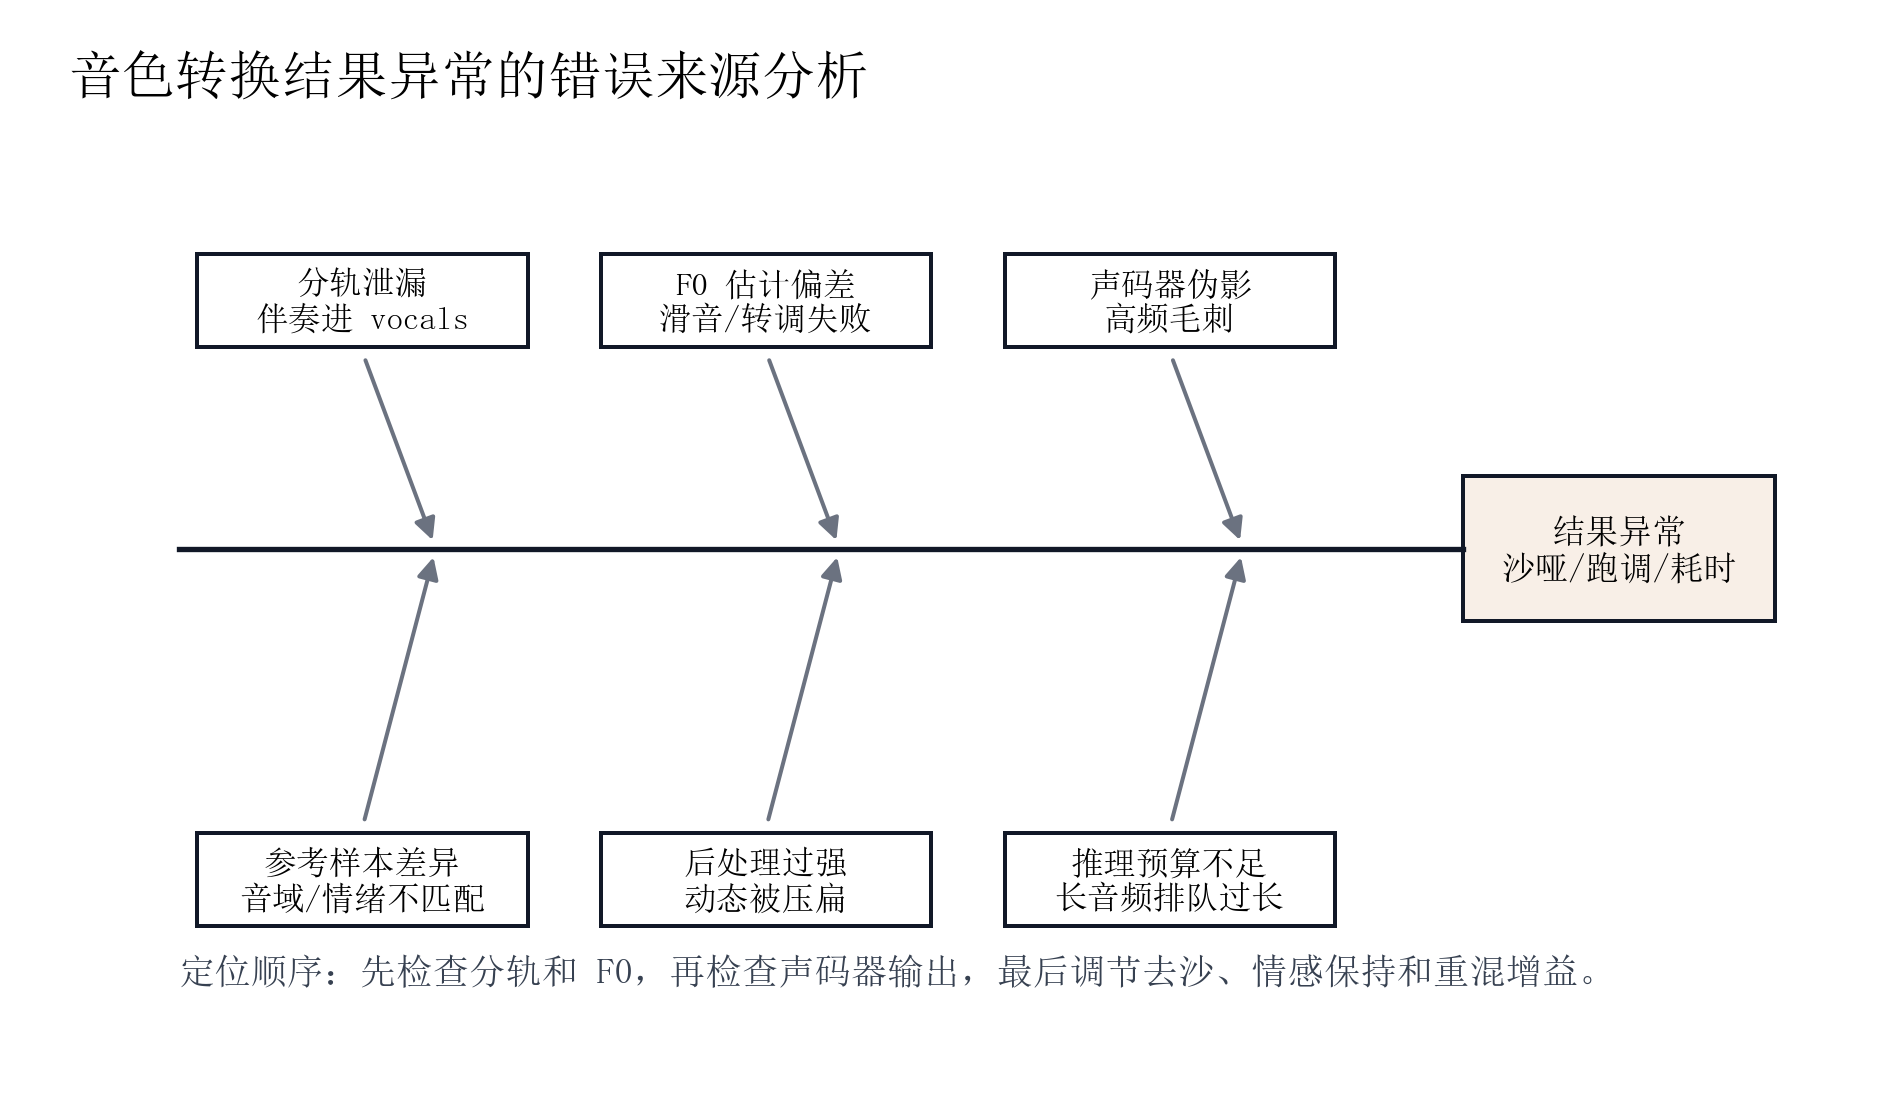
\includegraphics[width=0.92\linewidth]{assets/fig13_cn_error_source_analysis.png}
\caption{音色转换结果异常的错误来源分析。该图将沙哑、跑调、耗时和目标音色不稳定映射到可检查环节。}
\end{figure}
图14给出了本次段落级二次微调数据与 Mel 水印证据。左侧统计 15 秒训练片段的段落分布，右侧展示完整 Mel 图谱及其末尾频谱负形水印区域。水印段保持热谱图背景，“AI生成”由 Mel 矩阵中的低能量负形和高能量边缘显影共同形成。审阅者打开 png 可从谱图纹理中看到该标记，同时仍能观察整首音频从开始到结束的频谱能量变化。

\begin{figure}[H]
\centering
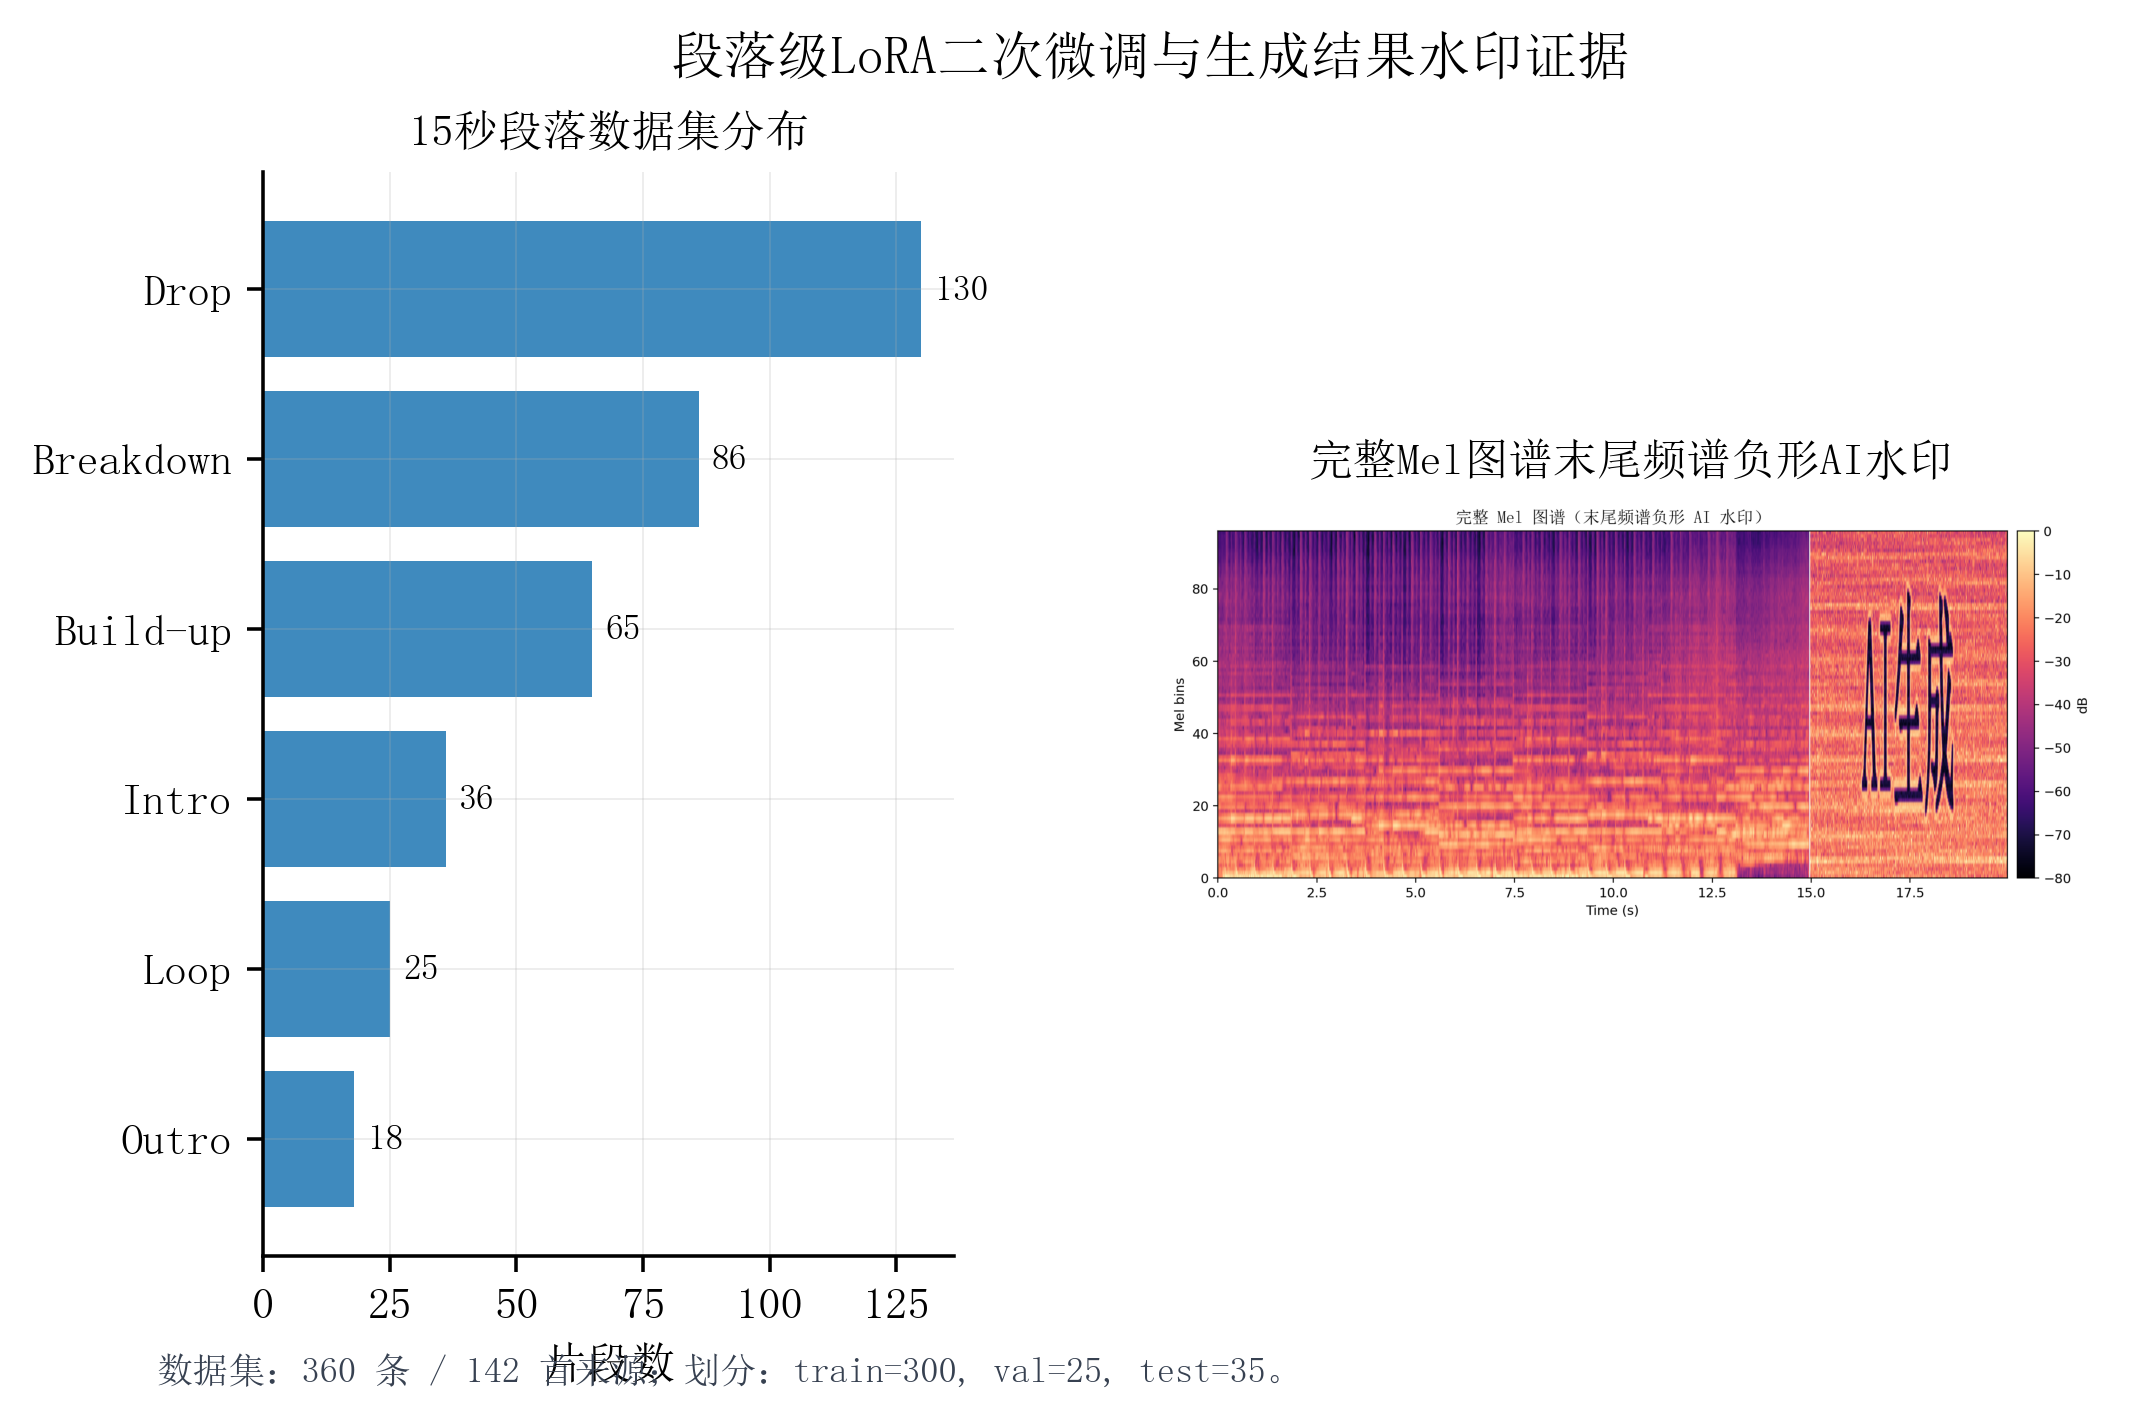
\includegraphics[width=0.92\linewidth]{assets/fig14_cn_section15_mel_watermark.png}
\caption{段落级LoRA二次微调与AI水印Mel证据。左侧为15秒段落数据集分布，右侧为完整Mel图谱末尾由低能量负形和高能量边缘显影形成的“AI生成”水印。}
\end{figure}
从工程实现看，跨环境调用 Demucs 是一个必要修正。网页进程与转换模型环境不一致时，若只在代码中捕获异常，用户只能看到“未产出 vocals”，无法判断是音频不可分离还是环境缺失。修复后的 wrapper 会在 base Python 缺少 demucs 时自动进入 edm-adapter 环境，并将四轨输出写回任务目录。这一处理提升了系统鲁棒性，也使论文中的分离与重混结果具有可验证来源。

\begin{table}[H]
\centering
\caption{当前局限与后续改进}
\small
\begin{tabular}{p{0.22\linewidth}p{0.32\linewidth}p{0.36\linewidth}}
\toprule
问题 & 当前表现 & 改进方向 \\
\midrule
推理速度 & 离线推理 RTF=19.30 & 增加分段预览、批处理缓存和高性能推理部署 \\
分轨质量 & 短片段可分离，完整歌曲仍依赖 Demucs 稳定性 & 加入分轨质量检测和 vocals 能量阈值 \\
评价指标 & 已有 BPM、RMS、低频比例、频谱和起音密度 & 增加音色相似度、人声清晰度和人工听评 \\
授权约束 & 目标音色以用户提供样本为条件 & 在网页端加入授权确认和数据来源记录 \\
\bottomrule
\end{tabular}
\end{table}
\section{结论}
本文构建了一个面向智能语音处理的音乐生成与授权歌声音色转换系统。系统在音乐生成侧使用 ACE-Step 和 LoRA 完成目标风格适配，在音色转换侧使用 Demucs 分离人声与伴奏，使用 Seed-VC 对 vocals 进行零样本音色替换，并将转换后人声与伴奏重混为新歌。实验部分给出了任务级证据链，包括分离音轨、重混输出、声学指标、频谱图、命令日志和 JSON 元数据。新增的控制变量矩阵、评价协议矩阵、长音频推理资源预算、去沙哑后处理链路和错误来源分析，使论文不仅展示系统能跑通，也解释了为什么需要分轨、为什么 TTS 不能替代 SVC、以及沙哑、情感不足和长音频资源开销问题应如何定位。结果说明，该系统已经形成从上传音频、智能分离、声线替换、伴奏重混到网页展示和论文报告的闭环。后续工作将重点优化推理部署效率、分轨质量评估、目标音色相似度量化和主观听评设计。

\section*{参考资料}
\begin{enumerate}[leftmargin=2em]
\item Ho J, Jain A, Abbeel P. Denoising Diffusion Probabilistic Models[C]//Advances in Neural Information Processing Systems. 2020.
\item Gong J, Zhao W, Wang S, Xu S, Guo J. ACE-Step: A Step Towards Music Generation Foundation Model[J/OL]. arXiv:2506.00045, 2025.
\item Hu E J, Shen Y, Wallis P, et al. LoRA: Low-Rank Adaptation of Large Language Models[C]//International Conference on Learning Representations. 2022.
\item Défossez A, Synnaeve G, Adi Y. Hybrid Spectrogram and Waveform Source Separation[C]//ISMIR Workshop, 2021.
\item Plachtaa. Seed-VC: zero-shot singing voice conversion toolkit[EB/OL]. GitHub repository, local clone: external\_tools/seed-vc.
\item Kong J, Kim J, Bae J. HiFi-GAN: Generative Adversarial Networks for Efficient and High Fidelity Speech Synthesis[C]//Advances in Neural Information Processing Systems. 2020.
\item Lee S, Ping W, Ginsburg B, Catanzaro B, Yoon S. BigVGAN: A Universal Neural Vocoder with Large-Scale Training[C]//International Conference on Learning Representations. 2023.
\item McFee B, Raffel C, Liang D, et al. librosa: Audio and Music Signal Analysis in Python[C]//Proceedings of the 14th Python in Science Conference. 2015.
\end{enumerate}
\end{document}